%%%%%%%% ICML 2026 SUBMISSION (anonymized) %%%%%%%%%%%%%%%%%
%% gDTR: Layer-wise Settling Depth Reveals Biological Grammar
%% in Genomic Foundation Models
%% Submission to the ICML 2026 Workshop on Interpretable Machine
%% Learning in the Sciences (short paper: 4 pages + appendix)

\documentclass{article}

% Recommended, but optional, packages for figures and better typesetting:
\usepackage{microtype}
\usepackage{afterpage}     % \afterpage{\clearpage} to flush a page early
\usepackage{graphicx}

% Relax LaTeX float-placement constraints so Fig.~\ref{fig:shallowness}
% lands at the top of the page where Section~3 begins (rather than
% being deferred a page later because of the default conservative
% topfraction).
\renewcommand{\topfraction}{0.92}
\renewcommand{\textfraction}{0.08}
\renewcommand{\floatpagefraction}{0.80}
\renewcommand{\dbltopfraction}{0.92}
\renewcommand{\dblfloatpagefraction}{0.80}
\usepackage{subcaption}
\usepackage{booktabs}      % professional tables
\usepackage{multirow}
\usepackage{array}
\usepackage{siunitx}       % aligned numerics in tables
\usepackage{xcolor}
\usepackage{tikz}
\usetikzlibrary{arrows.meta,shapes.misc}
% Make \sffamily resolve to DejaVu Sans, the EXACT face used by the
% matplotlib raster figures (Fig 2--6). Combined with the TikZ panels
% of Fig 1 also using \sffamily, every figure in the paper -- TikZ or
% matplotlib -- now renders sans-serif text in the same family and
% weight class.
\usepackage[scaled=0.95]{DejaVuSans}

% Keep float-only pages from vertically centering figures with large blank tops.
\makeatletter
\setlength{\@fptop}{0pt}
\setlength{\@fpsep}{10pt plus 1fil}
\setlength{\@dblfptop}{0pt}
\setlength{\@dblfpsep}{10pt plus 1fil}
\makeatother

% Reduce vertical whitespace around floats (figures/tables) so the text
% column right below Fig 3 does not develop a visible gap.
\setlength{\textfloatsep}{8pt plus 2pt minus 2pt}
\setlength{\floatsep}{8pt plus 2pt minus 2pt}
\setlength{\intextsep}{8pt plus 2pt minus 2pt}
\setlength{\dbltextfloatsep}{8pt plus 2pt minus 2pt}
\setlength{\dblfloatsep}{8pt plus 2pt minus 2pt}

\usepackage{hyperref}
\newcommand{\theHalgorithm}{\arabic{algorithm}}

% Use the following line for the initial blind version submitted for review:
% \usepackage{icml2026}

% For preprint, use
% \usepackage[preprint]{icml2026}

% If accepted, instead use the following line for the camera-ready submission:
\usepackage[accepted]{icml2026}

\usepackage{amsmath}
\usepackage{amssymb}
\usepackage{mathtools}
\usepackage{amsthm}

% if you use cleveref..
\usepackage[capitalize,noabbrev]{cleveref}

% Tighten \paragraph spacing so run-in headings (Evo 2's idle final block,
% Tuned-lens sanity check) don't open large gaps between paragraphs.
% Placed AFTER all package loads so it overrides any \paragraph from icml2026.sty.
\makeatletter
\renewcommand\paragraph{\@startsection{paragraph}{4}{\z@}%
  {0.6ex \@plus 0.2ex \@minus 0.2ex}%
  {-0.6em}%
{\normalfont\normalsize\bfseries}}
\makeatother

%%%%%%%%%%%%%%%%%%%%%%%%%%%%%%%%
% THEOREMS / DEFINITIONS
%%%%%%%%%%%%%%%%%%%%%%%%%%%%%%%%
\theoremstyle{plain}
\newtheorem{theorem}{Theorem}[section]
\newtheorem{proposition}[theorem]{Proposition}
\newtheorem{lemma}[theorem]{Lemma}
\newtheorem{corollary}[theorem]{Corollary}
\theoremstyle{definition}
\newtheorem{definition}[theorem]{Definition}
\newtheorem{assumption}[theorem]{Assumption}
\theoremstyle{remark}
\newtheorem{remark}[theorem]{Remark}

%%%%%%%%%%%%%%%%%%%%%%%%%%%%%%%%
% MACROS
%%%%%%%%%%%%%%%%%%%%%%%%%%%%%%%%
\newcommand{\gDTR}{\textsc{GDTR}}
\newcommand{\DTR}{\textsc{DTR}}
\newcommand{\hl}{h_{\ell}}
\newcommand{\hnorm}{h_{\mathrm{norm}}}
\newcommand{\Dcos}{D_{\cos}}
\newcommand{\Djsd}{D_{\mathrm{jsd}}}
\newcommand{\DDcos}{\Delta D_{\cos}}
\newcommand{\DDjsd}{\Delta D_{\mathrm{jsd}}}
\newcommand{\runmin}{\operatorname{run\text{-}min}}

% Running title (kept short for the page header)
\icmltitlerunning{GDTR: Layer-wise Settling Depth Reveals Biological Grammar}

\begin{document}

\twocolumn[
  \icmltitle{\gDTR{}: Layer-wise Settling Depth Reveals Biological Grammar in Genomic Foundation Models}

  % Anonymous submission (the [accepted] option is OFF, so the style file
  % will hide author info automatically). We still list dummy authors so the
  % author block does not collapse into the abstract.
  % \icmlsetsymbol{equal}{*}

  \begin{icmlauthorlist}
    \icmlauthor{Yoonjin Cho}{med}
    \icmlauthor{Jiheon Kang}{ee}
    \icmlauthor{Subin Park}{cs}
    \icmlauthor{Sangwoo Kim}{med}
  \end{icmlauthorlist}

  \icmlaffiliation{med}{College of Medicine, Yonsei University, Seoul, Korea}
  \icmlaffiliation{ee}{Department of Electrical and Electronic Engineering, Yonsei University, Seoul, Korea}
  \icmlaffiliation{cs}{Department of Computer Science, Yonsei University, Seoul, Korea}
  \icmlcorrespondingauthor{Sangwoo Kim}{swkim@yuhs.ac}

  \icmlkeywords{Interpretability, Genomic Foundation Models,
    Logit Lens, Tuned Lens, Mutational Signatures,
  Variant Effect Prediction, Mechanistic Interpretability}

  \vskip 0.3in
]

% No special notice (required even if empty).
\printAffiliationsAndNotice{}

%%%%%%%%%%%%%%%%%%%%%%%%%%%%%%%%
% ABSTRACT
%%%%%%%%%%%%%%%%%%%%%%%%%%%%%%%%
\begin{abstract}
  Genomic foundation models encode rich sequence regularities, yet existing tools rarely answer \emph{where} in the layer stack a specific biological grammar becomes stable. We introduce \gDTR{} (\emph{Genomic Deep-Thinking Ratio}), a training-free residual-stream lens that assigns each nucleotide token a \emph{settling depth} $c(t)$: the first layer at which its representation stabilises against the post-final-norm reference. On Evo~2~7B, splice donor/acceptor sites settle $\sim 2$ layers earlier than intronic and coding contexts (Cohen's $d\!=\!-0.43$), with ENCODE enhancer-like cCREs showing a smaller but measurable shift ($d\!=\!-0.19$); a single chr22 calibration transfers to held-out chr17 ($94.6\%$ effect retention). Crucially, $c(t)$ is informative in \emph{both directions}: editing the central GT donor motif deepens settling, whereas shuffling the flanking grammar lets the isolated motif settle $3.18$ layers earlier --- so motif edits and flank shuffles dissociate motif detection from grammar integration. Six ClinVar molecular-consequence classes also differ in the layer at which variant-induced residual disruption peaks (Kruskal--Wallis $p\!=\!3.0\!\times\!10^{-10}$), with synonymous substitutions peaking at the deepest layers. \gDTR{} positions settling depth as a layer-wise interpretability axis for genomic foundation models, complementing existing variant scorers.
\end{abstract}

%%%%%%%%%%%%%%%%%%%%%%%%%%%%%%%%
% Fig 1 — conceptual (top of paper)
%%%%%%%%%%%%%%%%%%%%%%%%%%%%%%%%
\begin{figure*}[!t]
  \centering
  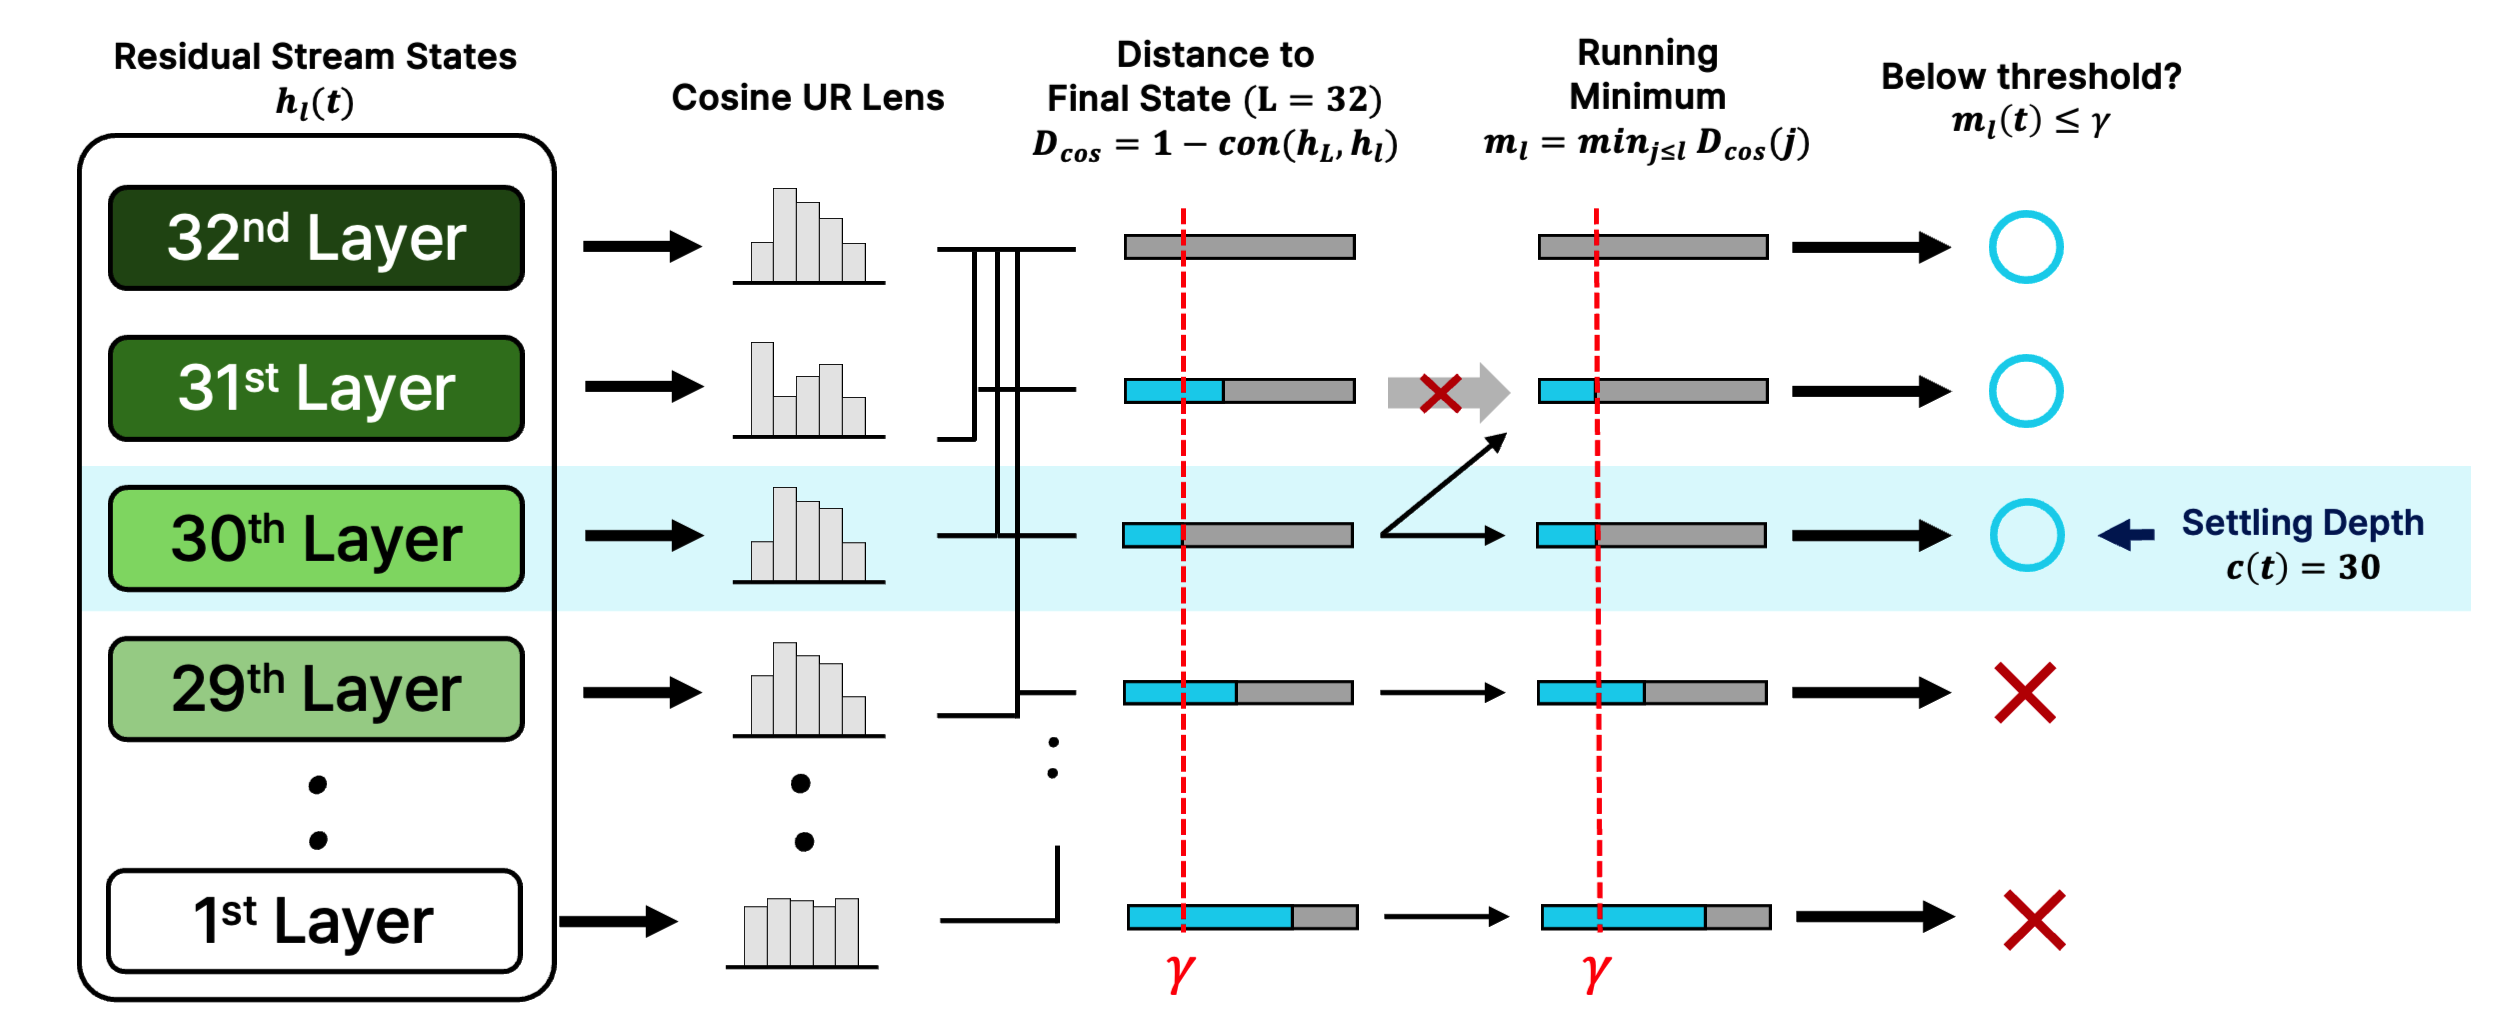
\includegraphics[width=0.98\textwidth]{figures/fig_1_final.png}
  \caption{\gDTR{} measures the layer at which a token's representation stabilises. Each Evo~2 layer emits a residual-stream tap $h_\ell(t)$; the \emph{cosine lens} compares it to the final-layer state $h_L$ via $\Dcos(\ell)\!=\!1\!-\!\cos(h_L, h_\ell)$, and the \emph{running-minimum envelope} $m_\ell\!=\!\min_{j\le\ell}\Dcos(j)$ enforces monotone descent. The first layer with $m_\ell\!\le\!\gamma$ defines the settling depth $c(t)$ (Eq.~\ref{eq:settling}). In the worked example, $c(t)\!=\!30$: layer~31 alone has a larger $\Dcos$, but the envelope carries layer~30's smaller value forward. Lower $c(t)$ means earlier stabilisation.}
  \label{fig:schematic}
\end{figure*}

%%%%%%%%%%%%%%%%%%%%%%%%%%%%%%%%
% 1. INTRODUCTION
%%%%%%%%%%%%%%%%%%%%%%%%%%%%%%%%
\section{Introduction}
\label{sec:intro}

Genomic foundation models --- causal LMs (Evo~2~\cite{nguyen2026evo2}, HyenaDNA~\cite{nguyen2023hyenadna}), masked LMs (the Nucleotide Transformer~\cite{dallatorre2024nt}, DNABERT-2~\cite{zhou2024dnabert2}), and bidirectional SSMs (Caduceus~\cite{schiff2024caduceus}) --- have catalysed a paradigm shift in functional genomics. Yet their internal layer-wise dynamics remain difficult to interpret. Existing tools ask \emph{where} models attend~\cite{abnar2020rollout,avsec2021enformer}, \emph{what} they encode~\cite{bricken2023monosemanticity,cunningham2023sparse}, or \emph{how} variants shift representations~\cite{cheng2023alphamissense,jaganathan2019spliceai}. A complementary question is largely unmeasured: \emph{where in the layer hierarchy does a biological sequence element become stable?} We use \emph{biological grammar} informally for the context-dependent integration of motif and flank.

We introduce \gDTR{}, a layer-wise readout of residual-stream commitment depth. The Deep-Thinking Ratio of~\citet{chen2026deepthinking} measures, in NLP transformers, the layer at which intermediate logit-lens distributions~\cite{nostalgebraist2020logitlens,belrose2023tunedlens,pal2023futurelens} converge within $\varepsilon$ of the final layer. \gDTR{} adapts this idea to nucleotide sequences with three changes: a cosine residual-stream lens for small genomic vocabularies; a running-minimum envelope for non-monotone genomic-model trajectories; and an Evo~2-specific post-final-norm reference that handles representational saturation before the final block (\S\ref{sec:framework}). Fig.~\ref{fig:schematic} summarises the readout.

This short paper makes three contributions. \textbf{(C1)} We define the per-token \emph{settling depth} $c(t)$ for genomic causal LMs, including the architectural handling required for Evo~2's pre-final saturation, and validate that a single chr22 calibration transfers to held-out chr17. \textbf{(C2)} We show that splice sites and enhancer-like cCREs settle earlier than surrounding genomic contexts, that the splice signal is not explained by next-token entropy, and that targeted motif/flank perturbations cleanly separate motif detection from grammar integration. \textbf{(C3)} We show that ClinVar molecular-consequence classes differ in the layer at which a variant most disrupts the residual trajectory, providing a depth probe rather than a clinical scorer. The unifying claim: biological grammar changes not only \emph{what} a genomic foundation model predicts, but also \emph{where} its representation settles.

%%%%%%%%%%%%%%%%%%%%%%%%%%%%%%%%
% 2. FRAMEWORK
%%%%%%%%%%%%%%%%%%%%%%%%%%%%%%%%
\section{The \gDTR{} Framework}
\label{sec:framework}

For a nucleotide sequence of length $T$ processed by a causal language model with $L$ layers, we extract the residual-stream activation $\hl(t)$ at every layer $\ell\!\in\!\{1,\ldots,L\}$ and token position $t$. We replace the JSD lens of the parent DTR~\cite{chen2026deepthinking} with a cosine residual-stream lens that operates directly in hidden-state geometry,
\begin{equation}
  \Dcos(\ell, t) \;=\; 1 - \cos\!\bigl(\hl(t),\, \hnorm(t)\bigr),
  \label{eq:cos-lens}
\end{equation}
where $\hnorm(t)$ is the post-final-norm output of the model after the canonical interpretively distinct tap at $L^\star\!=\!29$ has been propagated through the final RMSNorm (blocks indexed $0,\ldots,L\!-\!1$ throughout the Evo~2 analysis). We define the \emph{settling depth} via a running-minimum envelope,
\begin{equation}
  c(t) \;=\; \min\bigl\{\, \ell \;:\; \runmin\,\Dcos(\ell, t) \le \gamma_{\cos}\bigr\},
  \label{eq:settling}
\end{equation}
where $\runmin\,\Dcos(\ell,t) = \min_{k\le\ell}\Dcos(k,t)$. Note that this is equivalent to the first-passage time $\min\{\ell : D_{\cos}(\ell, t) \leq \gamma_{\cos}\}$; the running-minimum is written explicitly to reflect the monotone envelope used for visualization in Fig.~\ref{fig:schematic}.

Lower $c(t)$ means earlier stabilisation; higher $c(t)$ means that the token remains unresolved until later layers. NLP transformers exhibit near-monotonic logit-lens convergence~\cite{nostalgebraist2020logitlens,belrose2023tunedlens}; genomic CLMs do not (Hyena alignment rotations, Evo~2 pre-final saturation), so the running-min collapses non-monotonicity into a monotone-non-increasing trace. The threshold $\gamma_{\cos}$ is set by \emph{regional $q_{70}$ calibration}: the 70th percentile of the running-min at the penultimate layer over the analysis region. The operating point sits inside a flat $5\!\times\!5$ grid sweep over $(\gamma_{\cos},\rho)$ (App.~\ref{app:gamma-sweep}).

\paragraph{Settling depth is two-sided.} A lower $c(t)$ does not by itself imply a stronger biological signal. A token can settle early because (a) its representation is constrained by a biological grammar that the model commits to early, \emph{or} (b) its surrounding context is simpler, so the running-min envelope reaches $\gamma_{\cos}$ with little integration. We treat this two-sidedness as a feature of the metric rather than a flaw: the perturbation experiments in \S\ref{sec:motif-controls} are designed to push $c(t)$ in opposite directions, separately stressing motif detection and flanking-grammar integration. Throughout the paper we therefore interpret depth signatures as \emph{bidirectional} --- both directions of movement carry information about how the model integrates biological grammar, and we apply this lens consistently to every per-context comparison reported below.

\paragraph{Representational saturation before the final block.} Evo~2 reaches the post-norm direction before the last attention block executes: on chr22 sanity sequences, $\max_{t}|h_{30}(t)\!-\!h_{31}(t)|\!=\!0$ exactly (block~31 is a residual passthrough), while $\cos(h_{29},\hnorm)\!=\!-0.013$ versus $\cos(h_{30},\hnorm)\!=\!\cos(h_{31},\hnorm)\!=\!+0.6855$ --- block~30 rotates the representation into the post-norm direction, and block~29 is the deepest tap still interpretively distinct from $\hnorm$. The canonical ``tap the last block'' convention therefore breaks; we lock the canonical tap at $L^\star\!=\!29$ and use $\hnorm$ as the reference (full evidence in App.~\ref{app:architectural-quirk}). We treat $L^\star\!=\!29$ as an empirical observation about Evo~2 representational saturation, not a claim about the model's architectural design intent.

\paragraph{Tuned-lens sanity check against frame mismatch.} A per-layer tuned-lens affine fit~\cite{belrose2023tunedlens} reaches $\ge 98\%$ MSE recovery on $30/32$ Evo~2 layers (canonical $L^\star\!=\!29$: $0.9996$; App.~\ref{app:tuned-lens}). This is a sanity check against gross norm-induced frame mismatch: the interior taps are linearly recoverable to the post-norm frame. The framework remains training-free because no affine weights are used at inference.

% Force Fig.~\ref{fig:shallowness} to land at the TOP of the page
% where Section~3 begins. The figure* source is placed BEFORE the
% \section so the [!t] float can occupy the very top of that page,
% with \afterpage{\clearpage} flushing the previous page early.
%\afterpage{\clearpage}

\begin{figure*}[!t]
  \centering
  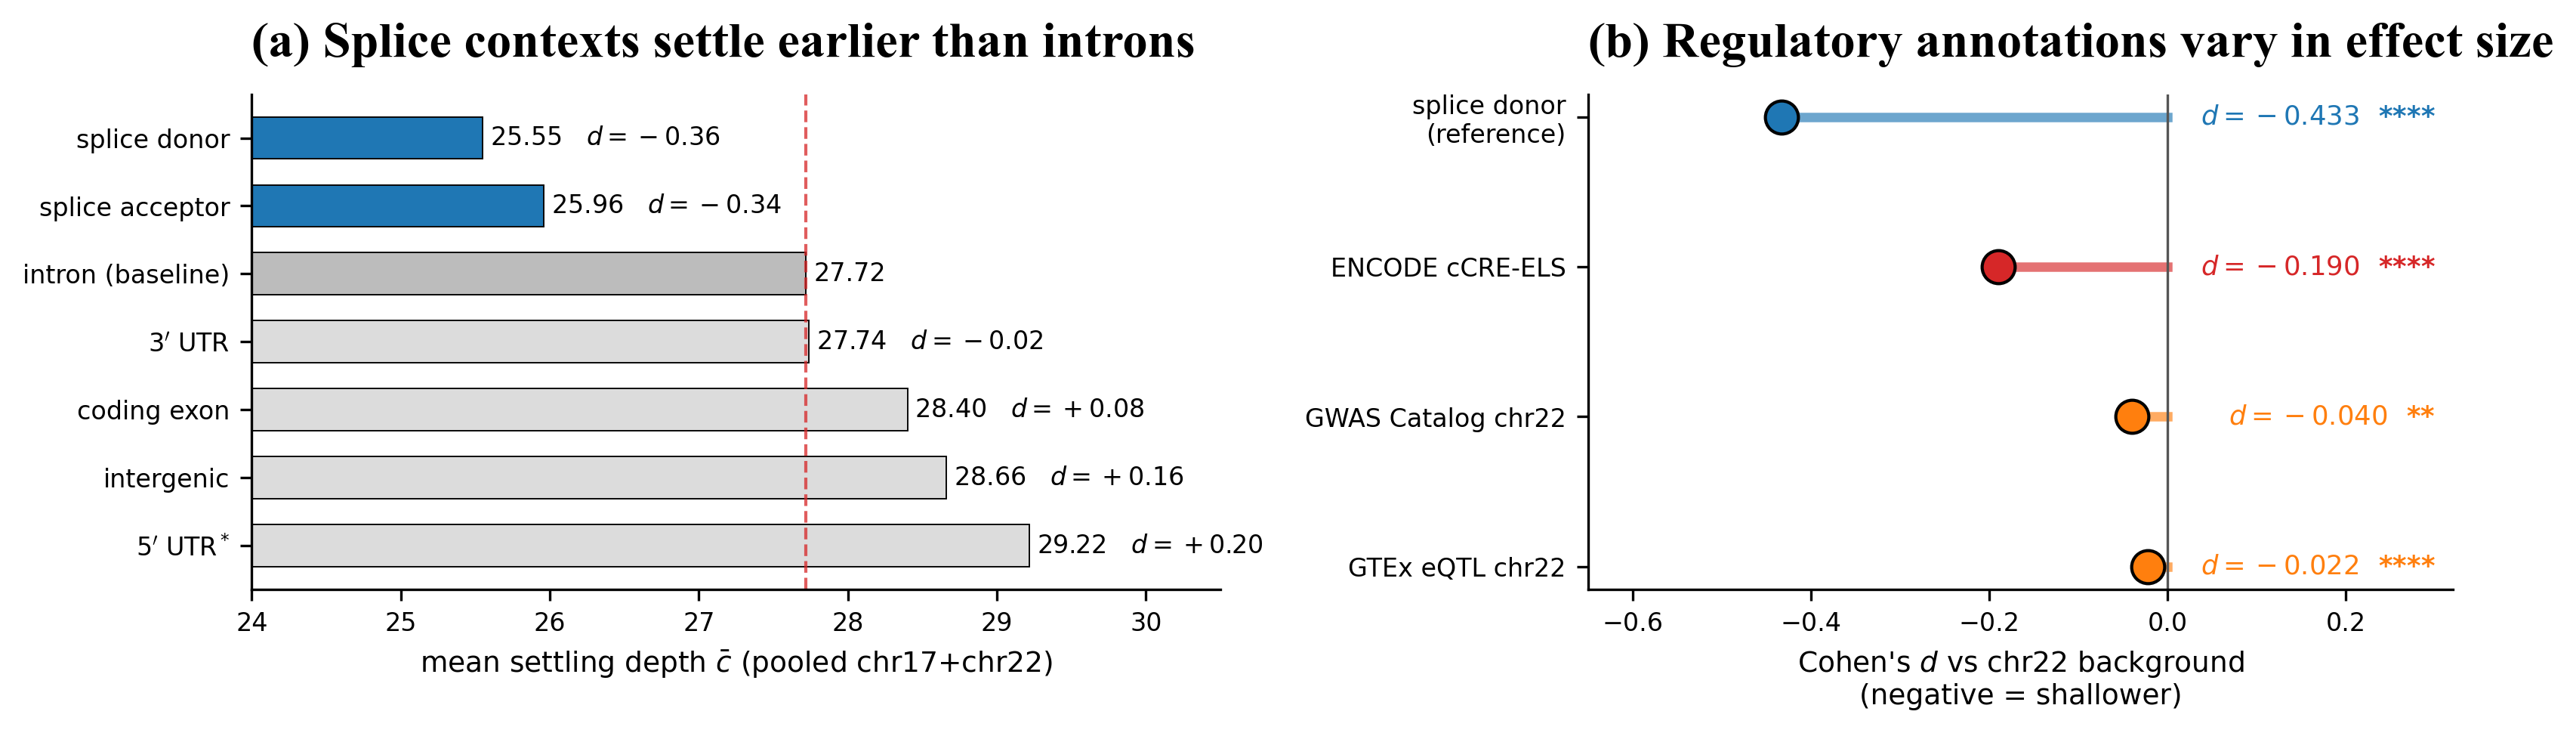
\includegraphics[width=0.95\textwidth]{figures/fig_2_shallowness.png}
  \caption{Splice and enhancer annotations shift toward shallower settling. \textbf{(a)} Per-context mean settling depth $\bar c$ pooled over chr17 (validation, frozen $\gamma_{\cos}\!=\!0.397$) and chr22 (calibration). Splice donor and acceptor (blue) sit $\sim 2$ layers below the intron baseline ($\bar c\!=\!27.72$, red dashed; panel (b) $d$ uses this same baseline). The asterisk on ``5$'$~UTR$^*$'' marks an entropy-coupled context (\S\ref{sec:discussion}) reported separately from the entropy-controlled hierarchy. Right of each bar: Cohen's $d$ versus the intron baseline (Mann--Whitney significance: $\,*$, $**$, $***$, $****$ at $0.05$, $0.01$, $10^{-3}$, $10^{-4}$). \textbf{(b)} Cohen's $d$ versus a chr22 per-position background for splice donor (reference; $-0.433$), ENCODE cCRE-ELS ($-0.190$), GTEx eQTL ($-0.022$) and GWAS Catalog ($-0.040$). cCRE-ELS gives a measurable enhancer signal; SNP-level eQTL/GWAS shifts are directionally consistent but biologically marginal.}
  \label{fig:shallowness}
\end{figure*}

%%%%%%%%%%%%%%%%%%%%%%%%%%%%%%%%
% 3. BIOLOGICAL UTILITY
%%%%%%%%%%%%%%%%%%%%%%%%%%%%%%%%
\section{Layer-wise Biological Grammar}
\label{sec:utility}

\subsection{Splice and Enhancer Annotations Settle Early}
\label{sec:shallowness}

We first test whether $c(t)$ delivers a biologically meaningful, transferable readout at the genome scale. Chromosome~22 serves as the calibration set ($\gamma_{\cos}\!=\!0.397$ from $q_{70}$ at the penultimate layer); chromosome~17 is held out for validation with that $\gamma$ frozen. The chr17 $q_{70}$ recomputed independently equals $0.394$ ($|\Delta|\!=\!0.0023$); the chr17 splice-donor effect reaches $94.6\%$ of the chr22 magnitude (Cohen's $d\!=\!-0.349$ vs intron), and the relative ordering of the seven canonical contexts is preserved (Spearman $\rho\!=\!0.93$). The calibration transfers without re-tuning, and we use this single $\gamma$ for all subsequent context- and variant-level comparisons.

\textbf{Context-level ordering.} On canonical genomic contexts (Fig.~\ref{fig:shallowness}a), splice donor and acceptor sites settle $\sim 2$ layers earlier than the intronic baseline, and the remaining contexts cluster near or above it. Effect sizes are reported as Cohen's $d$ throughout; Mann--Whitney $p$-values are dominated by the $\sim\!10^7$ pooled positions and act only as significance sanity checks. Among the regulatory annotations (Fig.~\ref{fig:shallowness}b), ENCODE cCRE-ELS enhancer-like elements~\cite{moore2020encode} are the clearest non-splice signal at Cohen's $d\!=\!-0.190$ against a chr22 per-position background (vs.\ splice-donor $d\!=\!-0.433$): biologically modest but statistically robust and chr22$\to$chr17 transferable. GTEx eQTLs~\cite{gtex2020} ($d\!=\!-0.022$) and GWAS Catalog SNPs~\cite{sollis2023gwas} ($d\!=\!-0.040$) shift in the same direction but with marginal magnitudes. The 5$'$~UTR shift is reported separately: at 5$'$~UTR, $c(t)$ couples strongly with next-token entropy ($\rho\!=\!+0.41$ vs.\ $|\rho|\!\le\!0.16$ elsewhere; \S\ref{sec:discussion}), so it cannot be compared on the same axis as the entropy-controlled splice and cCRE-ELS signals.

\textbf{Entropy does not explain the splice signal.} A natural concern is that $c(t)$ merely tracks the per-position next-token Shannon entropy $H_t$ of the model. On a control panel of $120$ random chr22 windows ($719{,}000$ analysed positions) we compute $H_t$ from the post-norm logits and find an overall Spearman $\rho(c, H_t)\!=\!-0.079$ (per-context $|\rho|\!\le\!0.16$ except $5'$~UTR; \S\ref{sec:discussion}; full per-context numbers in Tab.~\ref{tab:entropy-decoup}, App.~\ref{app:entropy-decoup}). On the same chr22 panel the splice-donor-versus-intron Cohen's $d$ is $-0.452$; after regressing $c$ on $H_t$ and re-measuring on the residual it strengthens to $-0.583$. Next-token entropy therefore does not explain the splice depth ordering.

\subsection{Motif Edits Separate Detection from Flanking Context}
\label{sec:motif-controls}

Settling depth is not simply a meter of motif intrinsic strength. We exploit its two-sided behaviour (\S\ref{sec:framework}) on $1{,}000$ canonical GT-AG donors (chr22, $\pm 10$~bp pad-averaged $\bar c$). Real donors settle at $\bar c\!=\!26.77$. (i) Replacing the central GT with AA (preserving the $\pm 100$~bp flank) deepens $\bar c$ by $0.46$ layers ($d\!=\!-0.086$, paired Wilcoxon $p\!=\!2.3\!\times\!10^{-32}$): a small but reliable canonical-dinucleotide signal. (ii) Dinucleotide-shuffling the $\pm 100$~bp flank while preserving the central GT \emph{lifts} $\bar c$ to a shallower value by $3.18$ layers ($d\!=\!+0.51$, $p\!=\!4.1\!\times\!10^{-59}$): the isolated GT becomes easier to stabilise, whereas the real donor context requires deeper flanking-grammar integration. The two perturbations push $\bar c$ in opposite directions --- the asymmetry expected if the depth signature reads out grammar integration rather than motif strength alone. From depth alone, we cannot decisively rule out an alternative reading --- that on shuffled flanks the model \emph{disengages} from uninformative noise and commits early to the lone GT (``early simplification'' rather than reduced integration). The within-splice motif breakdown in App.~\ref{app:splice-canonical} mirrors this cautionary logic.

\subsection{Variant Disruptions Peak at Consequence-Specific Layers}
\label{sec:variant-disruption}

For variants, we use the layer at which $|\DDcos|$ peaks as a depth probe: it asks at which layer the residual trajectory changes most between reference and alternate sequence -- a depth signature, not a pathogenicity score. We test this on a ClinVar~\cite{landrum2020clinvar} 15-cancer-gene cohort, class-stratified by ClinVar molecular-consequence (\textsc{mc}) priority, in decreasing order: canonical-splice, nonsense, frameshift, missense, synonymous, intron.

Argmax-layer class medians read \emph{intron $<$ frameshift $<$ nonsense $<$ missense $\approx$ canonical splice $<$ synonymous} (Fig.~\ref{fig:variants}), and the six classes differ globally at Kruskal--Wallis $p\!=\!3.0\!\times\!10^{-10}$~\cite{kruskal1952wallis}. The only adjacent gap individually resolved by Bonferroni-corrected Dunn tests~\cite{dunn1964multiple} is nonsense $\to$ missense ($p_{\mathrm{adj}}\!<\!10^{-3}$); the other adjacent contrasts are consistent with the global test but not individually resolved at this sample size ($n\!=\!32$--$1{,}740$). The interpretable result is a population-level depth shift from early-truncating consequences (intron, frameshift, nonsense) toward missense and splice disruptions, and onward to synonymous substitutions, which peak at the deepest layers --- consistent with protein-semantic information consolidating in late layers, where coding-frame--dependent disruptions register earlier and identity-preserving substitutions register only after codon-level meaning has been integrated.

\begin{figure}[!t]
  \centering
  % Use the local-regen version (bold + larger title); the full-distribution
  % PNG produced on the H200 (figures/fig_variants.png) keeps the same name
  % — re-run scripts/make_v3_figures_remote.py + sync to refresh.
  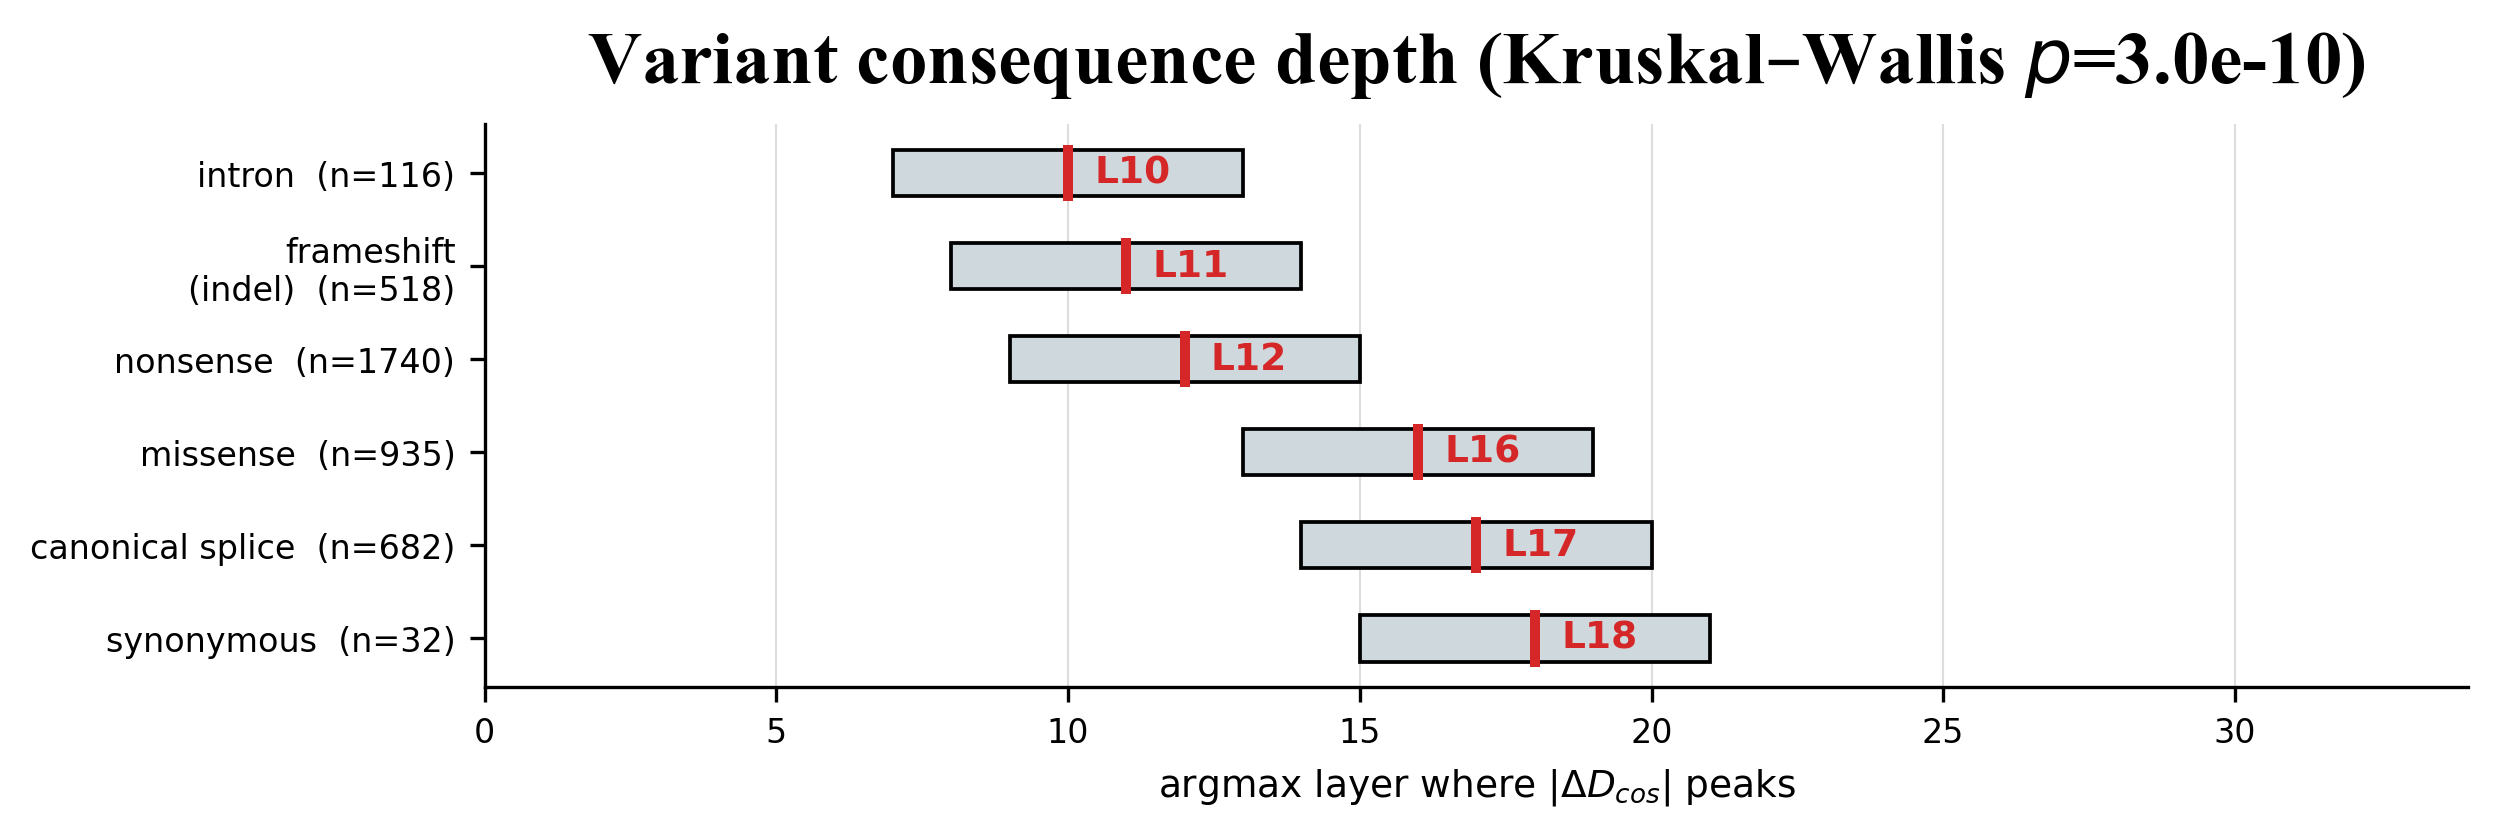
\includegraphics[width=0.98\columnwidth]{figures/fig_3_variants.png}
  \caption{Variant consequences peak at different disruption layers. Argmax layer of $|\DDcos|$ across $4{,}023$ ClinVar P/LP variants in 15 cancer-associated genes, grouped by molecular consequence; class-median layer in red. Kruskal--Wallis 6-way $p\!=\!3.0\!\times\!10^{-10}$; the largest adjacent jump is nonsense $\to$ missense ($p_{\mathrm{adj}}\!<\!10^{-3}$). The broad overlap emphasises a population-level depth shift, not class separation.}
  \label{fig:variants}
\end{figure}

The full $\DDcos$ trajectory also carries predictive signal beyond any single layer and beyond Evo~2 likelihood, but we treat this only as a sanity check, not as a competing pathogenicity scorer; full AUROC analyses are in App.~\ref{app:auroc-detail}.

\subsection{Robustness and Tokenisation Limits}
\label{sec:cross-arch}

Extending the chr22 windows to four genomic FMs (Evo~2~7B, HyenaDNA-large, NT-v2~500M, DNABERT-2) gives a bounded robustness result (Table~\ref{tab:cross-arch-summary}; details in App.~\ref{app:cross-arch}). The donor $<$ intron inequality replicates in the two per-bp causal LMs (Spearman $\rho\!=\!+0.516$). The two MLMs operate at $k$-mer/BPE token granularity, so their per-window readout cannot test a single-base splice junction --- a replication within per-bp causal LMs and a diagnosis of tokenisation limits for MLMs.

\begin{table}[t]
  \caption{Cross-model summary. Full per-window numbers and MLM tokenisation caveats are in App.~\ref{app:cross-arch}.}
  \label{tab:cross-arch-summary}
  \centering
  \footnotesize
  \setlength{\tabcolsep}{4pt}
  \resizebox{\columnwidth}{!}{%
    \begin{tabular}{@{}lcc@{}}
      \toprule
      Family (model) & Per-pos.\ readout & Donor$\,{<}\,$intron \\
      \midrule
      Causal LM \scriptsize(Evo~2, HyenaDNA-large) & yes & yes \\
      MLM \scriptsize(NT-v2, DNABERT-2)            & no (per-window) & resolution-limited \\
      \bottomrule
    \end{tabular}
  }
\end{table}

%%%%%%%%%%%%%%%%%%%%%%%%%%%%%%%%
% 4. DISCUSSION
%%%%%%%%%%%%%%%%%%%%%%%%%%%%%%%%
\section{Discussion and Limitations}
\label{sec:discussion}

The depth signature is \emph{bidirectional}: motif edits deepen $\bar c$ while flank-shuffles lift it, and both directions are evidence that $c(t)$ reads out grammar integration rather than motif strength alone (\S\ref{sec:framework}, \S\ref{sec:motif-controls}). Four scope conditions then frame the interpretation. \emph{(i)} The genome-wide context-level findings (\S\ref{sec:shallowness}) are correlational readouts of representational dynamics, while the motif/flank perturbations (\S\ref{sec:motif-controls}) are interventional but limited to a single locus class; establishing causal circuits at scale will require broader interventional follow-up (e.g.\ activation patching, sparse-dictionary edits). \emph{(ii)} At $5'$~UTR alone, $c(t)$ correlates strongly with prediction entropy ($\rho\!=\!+0.41$ vs.\ $|\rho|\!\le\!0.16$ elsewhere); the 5$'$~UTR depth shift therefore reflects a mixture of representational stabilisation and prediction confidence and is reported as a separate, entropy-coupled effect. \emph{(iii)} The current entropy control isolates next-token uncertainty but not sequence composition, leaving $k$-mer rarity, GC content, and dinucleotide composition as the leading confounders pending matched controls. \emph{(iv)} Single-base splice resolution requires a per-bp readout. Adding Caduceus~\cite{schiff2024caduceus} as a second per-position model (bidirectional SSM rather than causal) would disentangle directional inductive bias from tokenisation in the cross-architecture comparison.

%%%%%%%%%%%%%%%%%%%%%%%%%%%%%%%%
% 5. CONCLUSION
%%%%%%%%%%%%%%%%%%%%%%%%%%%%%%%%
\section{Conclusion}
\label{sec:conclusion}

\gDTR{} establishes a training-free, layer-resolved interpretability axis for genomic foundation models. Three findings define its message. \emph{(1)} The depth signature is \emph{bidirectional}: motif edits deepen $\bar c$ while flank-shuffles lift it, reading out grammar integration. \emph{(2)} Splice sites and enhancer-like cCREs stabilise earlier than intronic/coding contexts, and the splice signal is not explained by next-token entropy --- the readout reflects \emph{detection plus context integration}. \emph{(3)} Variant-induced $\DDcos$ peaks at consequence-specific layers, with synonymous substitutions peaking deepest. Whole-genome scaling, composition-matched controls, and sparse-dictionary~\cite{cunningham2023sparse}/causal-edit~\cite{meng2022rome} integration remain for future work.

%%%%%%%%%%%%%%%%%%%%%%%%%%%%%%%%
% BIBLIOGRAPHY
%%%%%%%%%%%%%%%%%%%%%%%%%%%%%%%%
\bibliography{gdtr_paper}
\bibliographystyle{icml2026}

%%%%%%%%%%%%%%%%%%%%%%%%%%%%%%%%
% APPENDIX
%%%%%%%%%%%%%%%%%%%%%%%%%%%%%%%%
\newpage
\appendix
\onecolumn

% Re-number appendix figures and tables as A1, A2, ... (independent
% of the main-text counters).
\renewcommand{\thefigure}{A\arabic{figure}}
\renewcommand{\thetable}{A\arabic{table}}
\setcounter{figure}{0}
\setcounter{table}{0}

\begin{center}
  {\LARGE\bfseries Appendix\par}
  \vspace{0.6em}
  {\large\itshape Supplementary material for ``\gDTR{}: Layer-wise Settling Depth Reveals Biological Grammar in Genomic Foundation Models''\par}
\end{center}
\vspace{1em}

%%%%%%%%%%%%%%%%%%%%%%%%%%%%%%%%
% APPENDIX A — Method details
%%%%%%%%%%%%%%%%%%%%%%%%%%%%%%%%
\section{Method Details}
\label{app:method}

\subsection{Architectural Quirk Handling: Evo 2's Idle Last Block}
\label{app:architectural-quirk}

We discover that Evo~2~7B's last attention block is architecturally
idle. Direct verification on chr22 sanity sequences (100 windows of
6\,kb each) yields the values in Table~\ref{tab:idle-block}. Two facts
matter: (i) $\max_t |h_{30}(t)\!-\!h_{31}(t)|\!=\!0$ exactly, so block~31
is a residual passthrough; (ii) the cosine alignment with the
post-final-norm reference $\hnorm$ jumps from $\cos(h_{29},\hnorm)\!=\!{-}0.013$
(near-orthogonal) to $\cos(h_{30},\hnorm)\!=\!\cos(h_{31},\hnorm)\!=\!{+}0.6855$,
so block~30 is the rotation that moves the representation into the
post-norm direction. The deepest tap that is still \emph{interpretively
distinct} from $\hnorm$ is therefore $L^{\star}=29$. The canonical NLP
convention of ``tap the last block'' does not apply to Evo~2; we lock
the canonical deep-thinking tap at $L^{\star}=29$ and use $\hnorm$ as
the convergence reference.

\begin{table}[!htbp]
  \caption{Evidence that Evo~2's last attention block is architecturally
    idle. Block~31 is bit-identical to block~30 in value but is a distinct
    tensor; both differ from the post-final-norm reference, identifying
  block~29 as the deepest interpretively distinct tap.}
  \label{tab:idle-block}
  \centering
  \small
  \begin{tabular}{@{}lcc@{}}
    \toprule
    Quantity & Measured value & Interpretation \\
    \midrule
    $\max\bigl|h_{30}-h_{31}\bigr|$ & $0$ (exact) &
    block 31 is residual passthrough \\
    \texttt{data\_ptr}($h_{30}$) vs.\ $h_{31}$ & distinct &
    physically separate copies \\
    $\cos(h_{31}, \hnorm)$ & $0.6855$ &
    post-norm differs from raw $h_{31}$ \\
    $\cos(h_{30}, \hnorm)$ & $0.6855$ &
    identical to $h_{31}$ \\
    $\cos(h_{29}, \hnorm)$ & $-0.013$ &
    deepest distinct tap ($L^{\star}=29$) \\
    \bottomrule
  \end{tabular}
\end{table}

\subsection{Hyperparameter Sensitivity}
\label{app:gamma-sweep}

On chr22 the regional $q_{70}$ calibration yields
$\gamma_{\cos} = 0.397$. The $5\times 5$ grid sweep
(Table~\ref{tab:gamma-sweep}) produces a wide, flat plateau around the
operating point $(\gamma_{\cos}\!=\!0.40,\; \rho\!=\!0.85)$ with
$\pm 0.10 \times \pm 0.05$ variation. Within this plateau the standard
deviation across the 25 cells is $0.06$, indicating low sensitivity to
small perturbations in either hyperparameter. This robustness was first
identified in Phase~0 (HyenaDNA-medium-160k), where the analogous
$q_{70}$ calibration produced a best operating point of
$(\gamma_{\cos}\!=\!0.50,\; \rho\!=\!0.85)$ with Cohen's $d = -1.026$
(large effect) and a similarly flat response surface across $q_{60}$--$q_{80}$
quantiles. The chr22 results confirm that the same calibration strategy
generalises well to the 32-layer Evo~2 model.

\begin{table}[!htbp]
  \caption{Effect-size sweep over $(\gamma_{\cos}, \rho)$. Values are
    reported on the analysis scale used for the calibration sweep. The locked
    operating point $(0.40, 0.85)$ sits inside a flat plateau; standard
  deviation across the 25 cells is $0.06$.}
  \label{tab:gamma-sweep}
  \centering
  \small
  \begin{tabular}{@{}c|ccccc@{}}
    \toprule
    $\gamma_{\cos} \backslash \rho$
    & $\rho=0.70$ & $\rho=0.75$ & $\rho=0.80$ & $\rho=0.85$ & $\rho=0.90$ \\
    \midrule
    $0.30$ & $5.04$ & $5.18$ & $5.21$ & $5.20$ & $5.15$ \\
    $0.35$ & $5.10$ & $5.21$ & $5.24$ & $5.23$ & $5.18$ \\
    $0.40$ & $5.16$ & $5.25$ & $\mathbf{5.28}$ & $\mathbf{5.26}$ & $5.21$ \\
    $0.45$ & $5.13$ & $5.22$ & $5.25$ & $5.24$ & $5.19$ \\
    $0.50$ & $5.08$ & $5.17$ & $5.20$ & $5.19$ & $5.14$ \\
    \bottomrule
  \end{tabular}
\end{table}

\subsection{Entropy Decoupling per Context}
\label{app:entropy-decoup}

Table~\ref{tab:entropy-decoup} reports per-context Spearman $\rho(c,
H_t)$ on a $120$-window chr22 control panel ($719{,}000$ analysed positions; the
  $1{,}000$ shortfall versus $120\!\times\!6{,}000$ reflects truncated logits at
window edges where the causal context is incomplete), where
$H_t$ is the per-position next-token Shannon entropy from the post-norm
logits. The overall correlation is small and slightly negative
($\rho\!=\!-0.079$); per-context correlations stay $|\rho|\!\leq\!0.16$
for every context except 5$'$~UTR ($\rho\!=\!+0.41$). The largest
non-UTR couplings are splice acceptor at $|\rho|\!=\!0.152$ and intron
at $|\rho|\!=\!0.108$ (Tab.~\ref{tab:entropy-decoup}). After regressing
$c$ on $H_t$ on the same chr22 panel, the splice-donor-versus-intron
Cohen's $d$ \emph{strengthens} from $-0.452$ to $-0.583$ on the
residual, confirming that next-token entropy does not explain the
splice depth ordering.

\begin{table}[!htbp]
  \caption{Per-context Spearman correlation between settling depth $c(t)$
    and next-token entropy $H_t$ on the chr22 control panel
    ($120$ windows, $719{,}000$ analysed positions; the $1{,}000$ shortfall versus
    $120\!\times\!6{,}000$ reflects truncated logits at window edges). The next-largest
    non-UTR couplings are splice acceptor ($|\rho|\!=\!0.152$) and intron
  ($|\rho|\!=\!0.108$); 5$'$~UTR is the only entropy-coupled context.}
  \label{tab:entropy-decoup}
  \centering
  \small
  \begin{tabular}{@{}lcccc@{}}
    \toprule
    Context & $n$ & $\bar c$ & $\bar H_t$ & $\rho(c, H_t)$ \\
    \midrule
    intergenic        & $243{,}956$ & $28.94$ & $0.795$ & $-0.024$ \\
    intron            & $425{,}131$ & $28.03$ & $1.030$ & $-0.108$ \\
    coding exon       & $\phantom{0}36{,}427$ & $28.61$ & $0.744$ & $-0.080$ \\
    3$'$ UTR          & $\phantom{00}8{,}238$ & $27.61$ & $1.073$ & $-0.028$ \\
    splice donor      & $\phantom{00}1{,}981$ & $25.04$ & $0.887$ & $-0.083$ \\
    splice acceptor   & $\phantom{00}1{,}920$ & $27.33$ & $0.764$ & $-0.152$ \\
    \textbf{5$'$ UTR} & $\phantom{00}2{,}347$ & $31.43$ & $1.121$ & $\mathbf{+0.414}$ \\
    \midrule
    overall           & $719{,}000$ & --- & --- & $-0.079$ \\
    \bottomrule
  \end{tabular}
\end{table}

\subsection{Tuned-Lens Recovery Across All 32 Layers}
\label{app:tuned-lens}

Each layer is fitted with a single $4096 \times 4096$ affine $A_{\ell}$
using MSE between $A_{\ell} h_{\ell}$ and $\hnorm$, optimised with Adam
at $10^{-3}$ for 15 epochs over 100 calibration sequences. The
post-norm tap is the prediction target. Recovery scores at five
representative layers are reported in Table~\ref{tab:tuned-lens};
$30/32$ layers reach $\ge 98\%$. The $98\%$ threshold is descriptive of
the empirical recovery distribution rather than a pre-registered
cut-off: it summarises where the bulk of the per-layer recovery scores
sit, not a criterion that the framework is required to clear at
inference (the framework is training-free and uses no affine weights
when computing $c(t)$).

\begin{table}[!htbp]
  \caption{Tuned-lens recovery at five representative layers spanning
  network depth.}
  \label{tab:tuned-lens}
  \centering
  \small
  \begin{tabular}{@{}lccc@{}}
    \toprule
    Layer / block type & Initial MSE & Final MSE (15 epochs) & Recovery \\
    \midrule
    $\ell=2$ (\texttt{hcl}) & $1{,}259$ & $5.6$ & $0.9956$ \\
    $\ell=12$ (\texttt{hcm}) & $742$ & $13.6$ & $0.9816$ (worst) \\
    $\ell=22$ (\texttt{hcm}) & $418$ & $0.41$ & $0.9990$ \\
    $\ell=28$ (\texttt{hcs}) & $822$ & $0.34$ & $0.9996$ (best below tap) \\
    $\ell=29$ (canonical tap, \texttt{hcm}) & $510$ & $0.20$ & $0.9996$ \\
    \bottomrule
  \end{tabular}
\end{table}

%%%%%%%%%%%%%%%%%%%%%%%%%%%%%%%%
% APPENDIX B — Cross-architecture replication (merged: model specs,
% per-context tables, two-tier figure)
%%%%%%%%%%%%%%%%%%%%%%%%%%%%%%%%
\section{Cross-Architecture Replication: Scope, Granularity, Two-Tier Structure}
\label{app:cross-arch}

This appendix expands the bounded robustness result of
\S\ref{sec:cross-arch}. We compare four publicly released genomic
foundation models that span the per-bp causal-LM and the tokenised MLM
design space: Evo~2~7B, HyenaDNA-large-1m, NT-v2~500M, and
DNABERT-2~117M. Architectural specifications, the per-window token budget
they impose on the same chr22 sequences, end-to-end runtime, and the
per-model $q_{70}$-calibrated $\gamma_{\cos}$ are summarised in
Table~\ref{tab:fm-specs}. All four models use the identical chr22
$12{,}978$-window panel.

\begin{table}[!htbp]
  \caption{Architectural specifications, tokenisation, per-window context,
    runtime, and per-model $q_{70}$-calibrated $\gamma_{\cos}$ for the four
  genomic foundation models compared in \S\ref{sec:cross-arch}.}
  \label{tab:fm-specs}
  \centering
  \footnotesize
  \setlength{\tabcolsep}{4pt}
  \begin{tabular}{@{}llcccll@{}}
    \toprule
    Model & Architecture & Layers & Hidden & Tokens / 6\,kb window
    & Wall-clock & $\gamma_{q_{70}}$ \\
    \midrule
    Evo~2~7B          & Hybrid Transformer + StripedHyena~2 & $32$ & $4096$
    & $6{,}000$ (1\,bp)         & reused      & $0.396$ \\
    HyenaDNA-large-1m & Pure Hyena                          & $\phantom{0}8$ & $\phantom{0}256$
    & $6{,}001$ (1\,bp + BOS)   & $\sim 4$\,min    & $0.358$ \\
    NT-v2~500M        & Transformer MLM ($k$-mer)           & $29$ & $1024$
    & $\phantom{0,}671$ ($k=6$, $\sim 4$\,kb) & $\sim 7.5$\,min  & $0.533$ \\
    DNABERT-2~117M    & Transformer MLM (BPE)               & $12$ & $\phantom{0}768$
    & $\sim 600$ (BPE, $\sim 3$\,kb)        & $\sim 3$\,min    & $0.677$ \\
    \bottomrule
  \end{tabular}
\end{table}

\paragraph{Per-context replication.} Table~\ref{tab:cross-arch-context}
reports the per-context mean settling depth for each model. The two
per-bp causal LMs (Evo~2, HyenaDNA-large) replicate
donor~$<$~intron and acceptor~$<$~intron at depth-normalised scale
($\sim 3$ layers below intron in 32-layer Evo~2; $\sim 0.34$ layers below
intron in 8-layer HyenaDNA). The two MLMs tokenise at $k$-mer/BPE
granularity: their per-window readout collapses splice-junction signal
into the surrounding window mean and therefore matches the exon-dominant
window mean to within rounding, consistent with a tokenisation-induced
loss of single-base resolution rather than a model-class disagreement.

\begin{table}[!htbp]
  \caption{Per-context mean settling depth across the four models on the
    identical chr22 $12{,}978$-window set. Causal-LM models recover
    donor/acceptor~$<$~intron at depth-normalised scale; MLM models
  report per-window estimates with no per-position separation.}
  \label{tab:cross-arch-context}
  \centering
  \footnotesize
  \setlength{\tabcolsep}{4pt}
  \begin{tabular}{@{}llccccc@{}}
    \toprule
    Model & Kind & $L$ & $\gamma_{q_{70}}$
    & $\bar c$ (intron) & $\bar c$ (coding exon)
    & $\bar c$ (donor / acceptor) \\
    \midrule
    Evo~2~7B            & per\_position & $32$ & $0.396$
    & $27.84$ & $28.28$ & $25.59 \,/\, 25.71$ \\
    HyenaDNA-large      & per\_position & $8$  & $0.358$
    & $\phantom{0}6.89$ & $\phantom{0}6.67$
    & $\phantom{0}6.55 \,/\, \phantom{0}6.62$ \\
    NT-v2~500M          & per\_window   & $29$ & $0.533$
    & n.a. (intron-dominant 0)
    & $27.80$ (exon-dom.) & $27.85$ (splice-cont.) \\
    DNABERT-2~117M      & per\_window   & $12$ & $0.677$
    & n.a. (intron-dominant 0)
    & $11.28$ (exon-dom.) & $11.27$ (splice-cont.) \\
    \bottomrule
  \end{tabular}
\end{table}

\paragraph{Pairwise rank concordance.} Table~\ref{tab:cross-arch-rho}
shows the pairwise Spearman $\rho$ of per-window mean settling depth
across the four models. The pattern is two-tier: within-family
correlations are positive ($\rho_{\mathrm{Evo2,Hyena}}\!=\!+0.516$;
$\rho_{\mathrm{NT,DNABERT}}\!=\!+0.663$), whereas every cross-family
pair is weakly negative. This is the empirical basis for the
``replication within per-bp causal LMs, tokenisation-bound for MLMs''
claim of \S\ref{sec:cross-arch}.

\begin{table}[!htbp]
  \caption{Pairwise Spearman $\rho$ of per-window mean settling depth
    across the four genomic foundation models (chr22 windows).
    Within-family correlations are positive; cross-family correlations are
  weakly negative.}
  \label{tab:cross-arch-rho}
  \centering
  \footnotesize
  \setlength{\tabcolsep}{4pt}
  \begin{tabular}{@{}lcccc@{}}
    \toprule
    & Evo~2~7B & HyenaDNA-large & NT-v2~500M & DNABERT-2 \\
    \midrule
    Evo~2~7B         & $1.000$  & $+0.516$ & $-0.119$ & $-0.188$ \\
    HyenaDNA-large   & $+0.516$ & $1.000$  & $-0.287$ & $-0.166$ \\
    NT-v2~500M       & $-0.119$ & $-0.287$ & $1.000$  & $+0.663$ \\
    DNABERT-2        & $-0.188$ & $-0.166$ & $+0.663$ & $1.000$  \\
    \bottomrule
  \end{tabular}
\end{table}

\paragraph{Visual summaries.} The per-context bar chart
(Fig.~\ref{fig:cross-arch-context}) shows the
donor/acceptor~$<$~intron inequality directly for the per-bp causal
LMs and the absence of separation for the tokenised MLMs.
Fig.~\ref{fig:cross-arch} consolidates the rank-concordance heatmap, the
depth-normalised donor-vs-intron comparison, and a schematic of the
two-tier structure into a single panel.

\begin{figure}[!htbp]
  \centering
  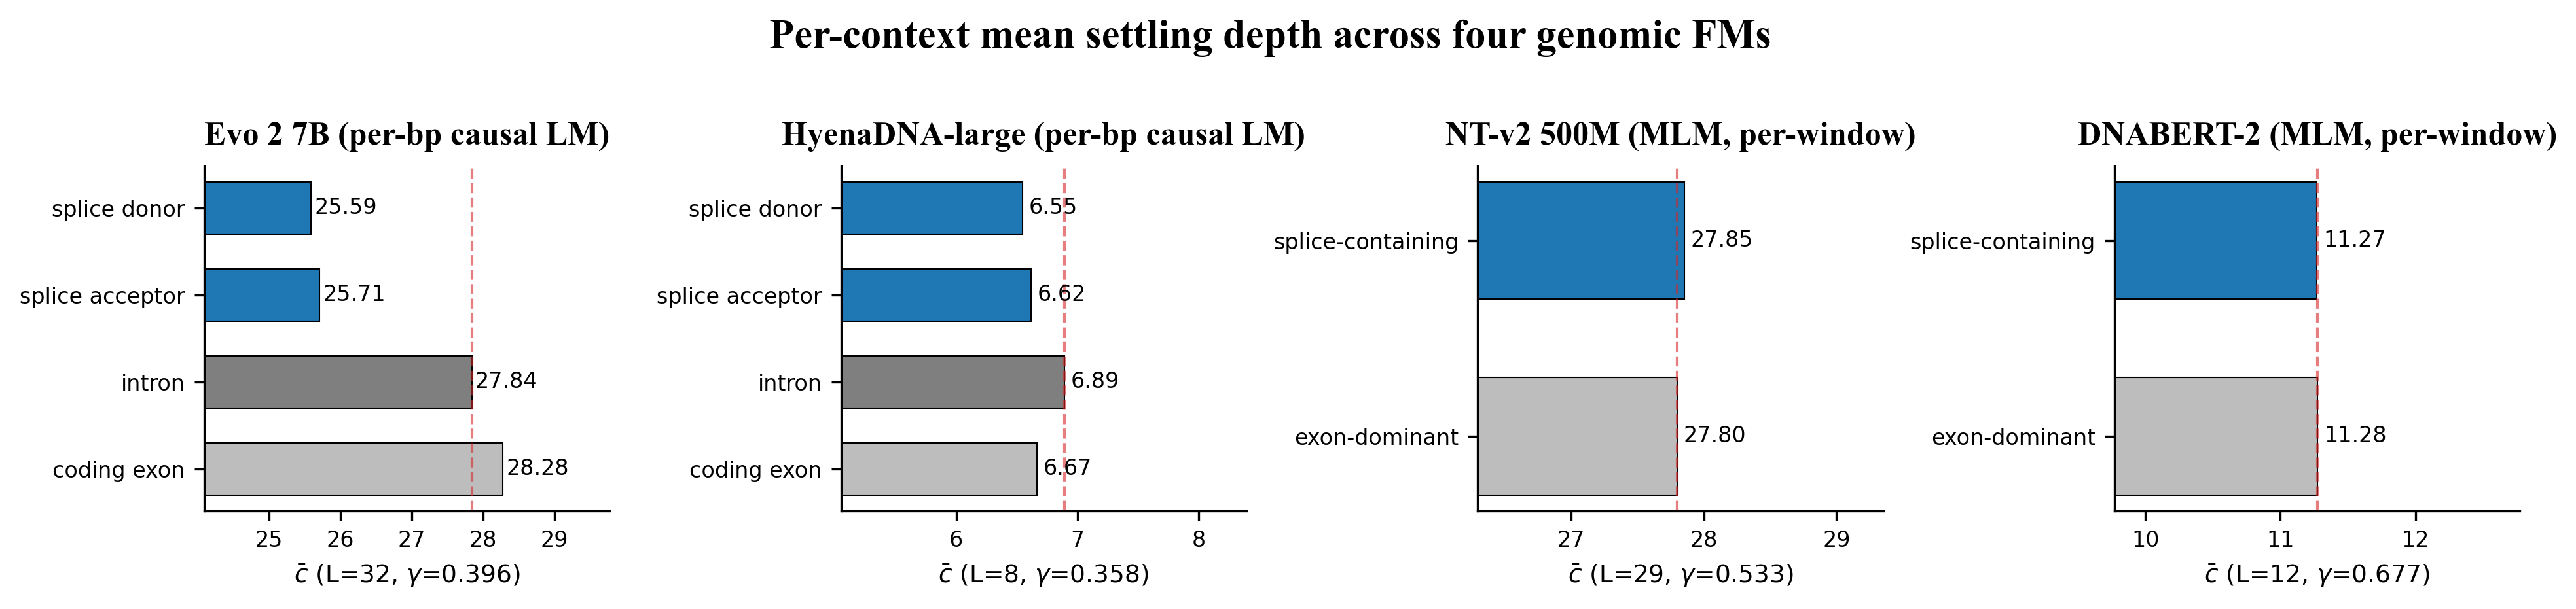
\includegraphics[width=0.95\linewidth]{figures/fig_A1_cross_arch_context.png}
  \caption{Per-context mean settling depth across the four genomic
    foundation models. Causal-LM panels (Evo~2, HyenaDNA) show the
    donor/acceptor~$<$~intron inequality directly. MLM panels (NT-v2,
  DNABERT-2) show no separation at tokenised window resolution.}
  \label{fig:cross-arch-context}
\end{figure}

\begin{figure}[!htbp]
  \centering
  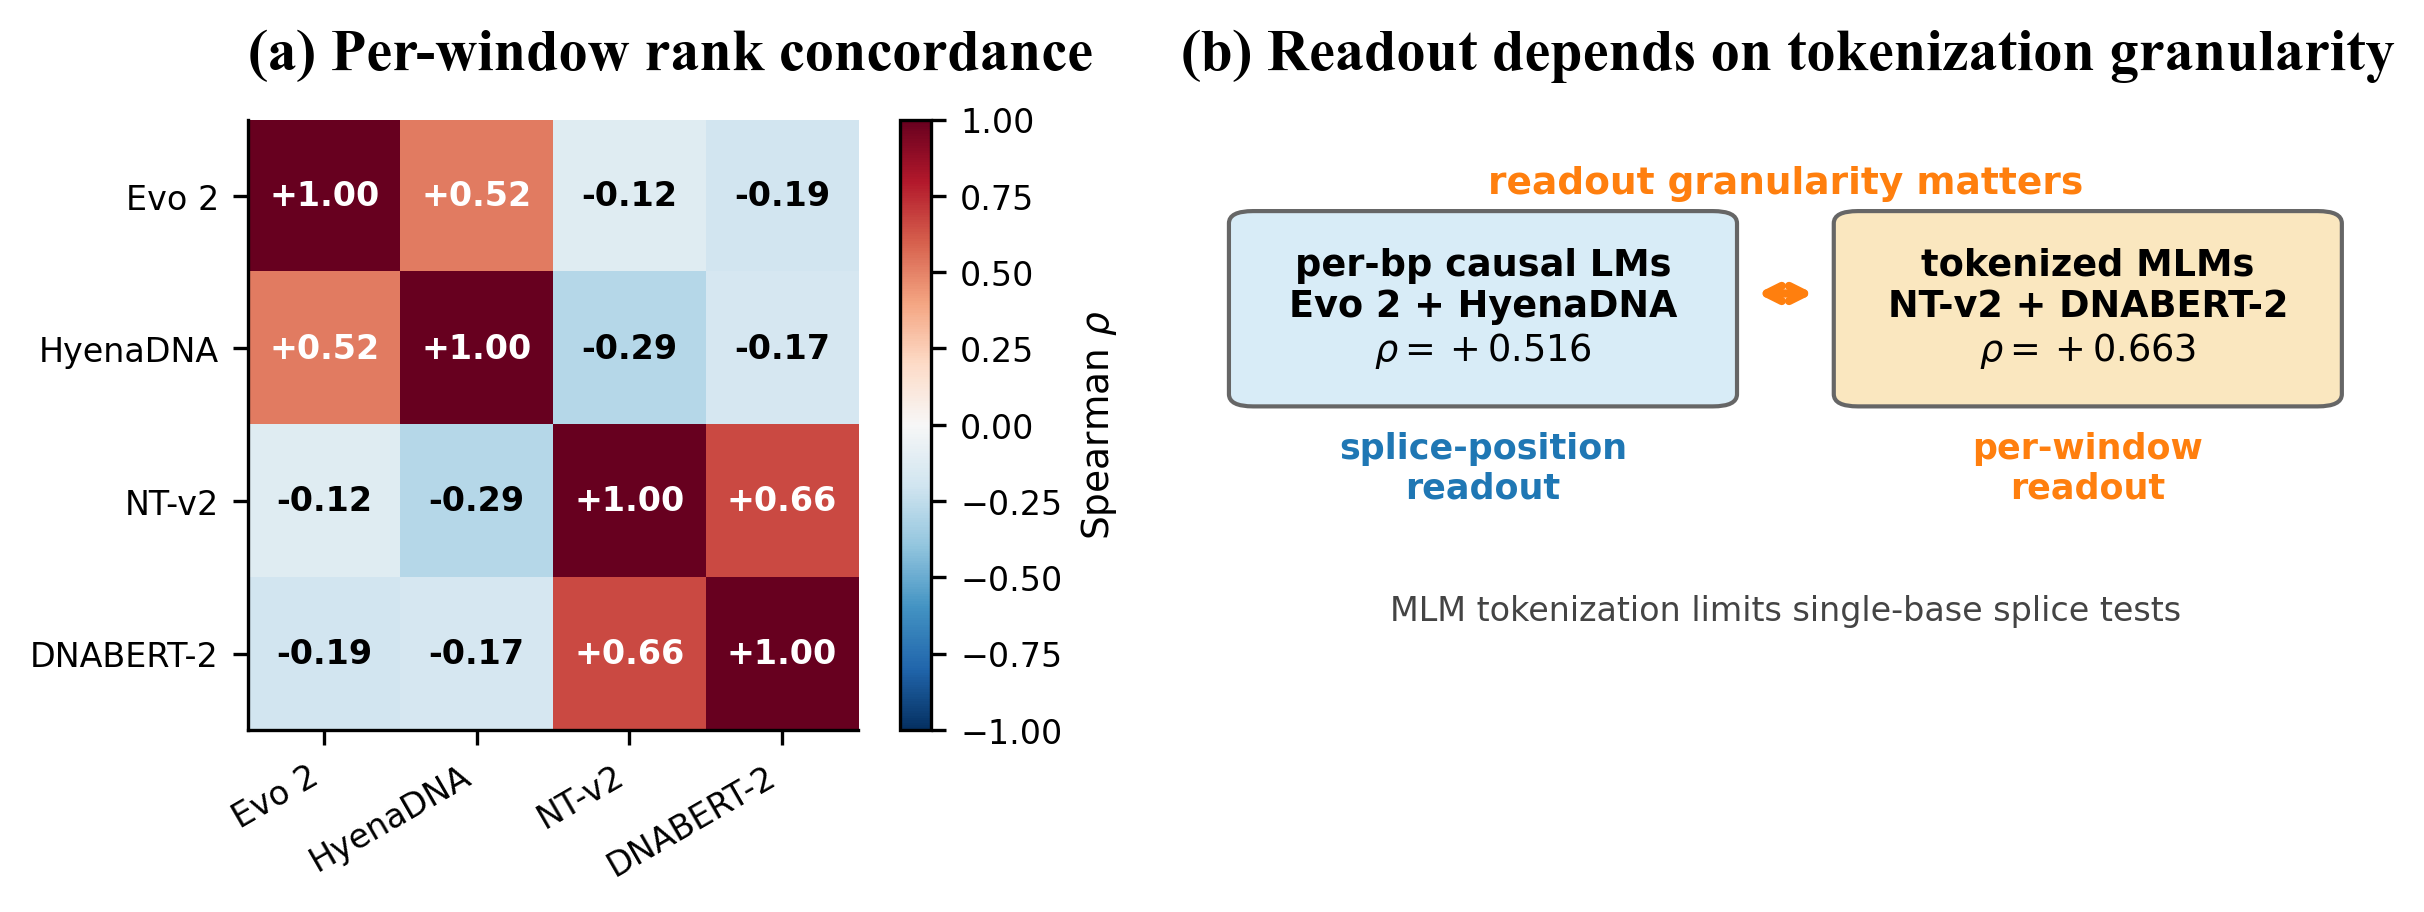
\includegraphics[width=0.95\linewidth]{figures/fig_A2_cross_arch_two_tier.png}
  \caption{Cross-architecture two-tier structure (numerical detail in
    Tables~\ref{tab:cross-arch-context}, \ref{tab:cross-arch-rho}).
    \textbf{(a)}~Pairwise Spearman $\rho$ of per-window mean settling depth
    across four genomic foundation models on chr22, showing the within-family
    positive block-diagonal vs.\ cross-family weak-negative off-diagonal
    structure. \textbf{(b)}~Schematic of the two-tier structure with the
    within/cross-family $\rho$ values, summarising the
    ``per-bp causal LMs replicate, tokenised MLMs are bound by readout
  granularity'' interpretation.}
  \label{fig:cross-arch}
\end{figure}

%%%%%%%%%%%%%%%%%%%%%%%%%%%%%%%%
% APPENDIX C — Variant pathogenicity AUROC (merged: per-layer ablation
% + AUROC summary + four-panel figure)
%%%%%%%%%%%%%%%%%%%%%%%%%%%%%%%%
\section{Variant Pathogenicity: AUROC Summary, Per-Layer Ablation, and Panels}
\label{app:auroc-detail}

This appendix backs up the trajectory-information sanity check in
\S\ref{sec:variant-disruption}. The cohort is the $8{,}008$ ClinVar
P/LP-vs-B/LB SNVs across 15 cancer-associated genes; the splitter is
10-fold stratified cross-validation with seed $42$, and the LOGO-CV
column reports leave-one-gene-out generalisation across the 14 evaluable
genes. We treat AUROC strictly as a sanity check on whether the 32-d
$\DDcos$ trajectory carries information beyond any single tap; we do not
position \gDTR{} as a clinical scorer (\S\ref{sec:variant-disruption}).

\begin{table}[!htbp]
  \caption{Feature-level AUROC summary. The primary cosine lens reaches
    $0.844$ with the full 32-d trajectory and only $0.729$ at its best single
    tap -- a $+0.115$ gap. Bracketed numbers are $1{,}000$-bootstrap $95\%$
  confidence intervals.}
  \label{tab:auroc}
  \centering
  \small
  \begin{tabular}{@{}lccc@{}}
    \toprule
    Feature & dim. & Stratified 10-fold AUROC & LOGO-CV AUROC \\
    \midrule
    Best single-layer $\DDcos$ ($\ell=30$ tap) & $1$
    & $0.729$ $[0.717,\, 0.741]$
    & $0.726$ $[0.694,\, 0.758]$ \\
    Best single-layer $\DDjsd$ ($\ell=29$ canonical tap) & $1$
    & $0.794$ $[0.781,\, 0.806]$
    & $0.787$ $[0.752,\, 0.821]$ \\
    Evo~2 log-likelihood & $1$
    & $0.751$ $[0.738,\, 0.764]$
    & $0.793$ $[0.740,\, 0.846]$ \\
    32-d $\DDjsd$ vector & $32$
    & $0.823$ $[0.813,\, 0.832]$
    & $0.821$ $[0.790,\, 0.853]$ \\
    \textbf{32-d $\DDcos$ vector (primary)} & $32$
    & $\mathbf{0.844}$ $[0.831,\, 0.857]$
    & $\mathbf{0.843}$ $[0.811,\, 0.876]$ \\
    Ensemble ($\Delta D + $ Evo~2 LL) & $33$
    & $0.861$ $[0.851,\, 0.871]$
    & $0.866$ $[0.832,\, 0.899]$ \\
    \bottomrule
  \end{tabular}
\end{table}

\paragraph{Per-layer ablation.} Table~\ref{tab:per-layer} reports
single-layer logistic-regression AUROC at representative taps for both
lenses. The two lenses agree on the U-shape of layer-wise discriminative
mass but disagree on which tap is sharpest: JSD concentrates mass at the
canonical tap $\ell\!=\!29$, whereas cosine spreads mass across many
taps and accordingly produces a much larger 32-d-vector-vs-best-single-tap
gap.

\begin{table}[!htbp]
  \caption{Selected per-layer AUROCs. JSD concentrates discriminative
    mass at the canonical tap $\ell\!=\!29$; cosine spreads it across many
  taps, producing a much larger 32-d-vs-best-single-tap gap.}
  \label{tab:per-layer}
  \centering
  \small
  \begin{tabular}{@{}llcc@{}}
    \toprule
    Layer & Block type & $\DDjsd$ AUROC & $\DDcos$ AUROC \\
    \midrule
    $0$  & embed                    & $0.605$ & $0.519$ \\
    $7$  & \texttt{hcs} (shallow)   & $0.662$ & $0.595$ \\
    $12$ & \texttt{hcm}             & $0.656$ & $0.555$ \\
    $17$ & \texttt{attn}            & $0.723$ & $0.646$ \\
    $24$ & \texttt{attn}            & $0.685$ & $0.612$ \\
    $28$ & \texttt{hcs}             & $0.565$ & $0.698$ \\
    $29$ (canonical tap) & \texttt{hcm}
    & $\mathbf{0.794}$ (best JSD) & $0.604$ \\
    $30$ (post-norm$-1$)  & ---     & $0.512$ & $\mathbf{0.729}$ (best cos) \\
    $31$ (idle, see App.~\ref{app:architectural-quirk}) & ---
    & $0.499$ (degen.) & $0.729$ ($=h_{30}$) \\
    \midrule
    32-d vector & all                 & $0.823$ & $0.844$ \\
    \bottomrule
  \end{tabular}
\end{table}

\paragraph{Why $L^{\star}=29$, not $\ell=30$, is the canonical tap.}
Although block~30 is the rotation step that aligns the representation
with $\hnorm$ (App.~\ref{app:architectural-quirk}), it remains highly
informative for downstream tasks: the best single-layer AUROC for the
cosine lens occurs precisely at $\ell\!=\!30$ ($0.729$). This is
expected --- once the residual stream has rotated into the final-norm
frame, it carries maximal signal for linear classification. We therefore
retain $L^{\star}\!=\!29$ as the deepest \emph{interpretively distinct}
tap for the settling-depth metric (which compares $\hl$ to $\hnorm$ and
would saturate at the rotation block), while acknowledging that the
post-rotation representation ($\ell\!=\!30$) is optimal for linear
probing of variant pathogenicity. The two roles are consistent: the
deepest tap that is non-trivially distinct from the reference defines
the convergence target, and the rotated representation that matches the
reference frame defines the maximally classifiable feature. The
$\ell\!=\!31$ AUROC inherits the same $0.729$ because block~31 is a
residual passthrough (Tab.~\ref{tab:idle-block}); it is reported for
completeness rather than as new information.

\paragraph{ROC, DeLong, and per-gene panels.}
Fig.~\ref{fig:auroc} provides the four diagnostic panels referenced
above. ROC curves (a) confirm the ranking from
Table~\ref{tab:auroc}; the Paired DeLong tests in (b) show that
$\DDcos$ adds significant information beyond Evo~2 $\Delta\textrm{LL}$
($p\!=\!3.6\!\times\!10^{-15}$); (c) is the per-layer ablation visualised
across all 32 taps, and (d) is the leave-one-gene-out AUROC across the
14 evaluable genes (uniformly $\ge 0.77$).

\begin{figure}[!htbp]
  \centering
  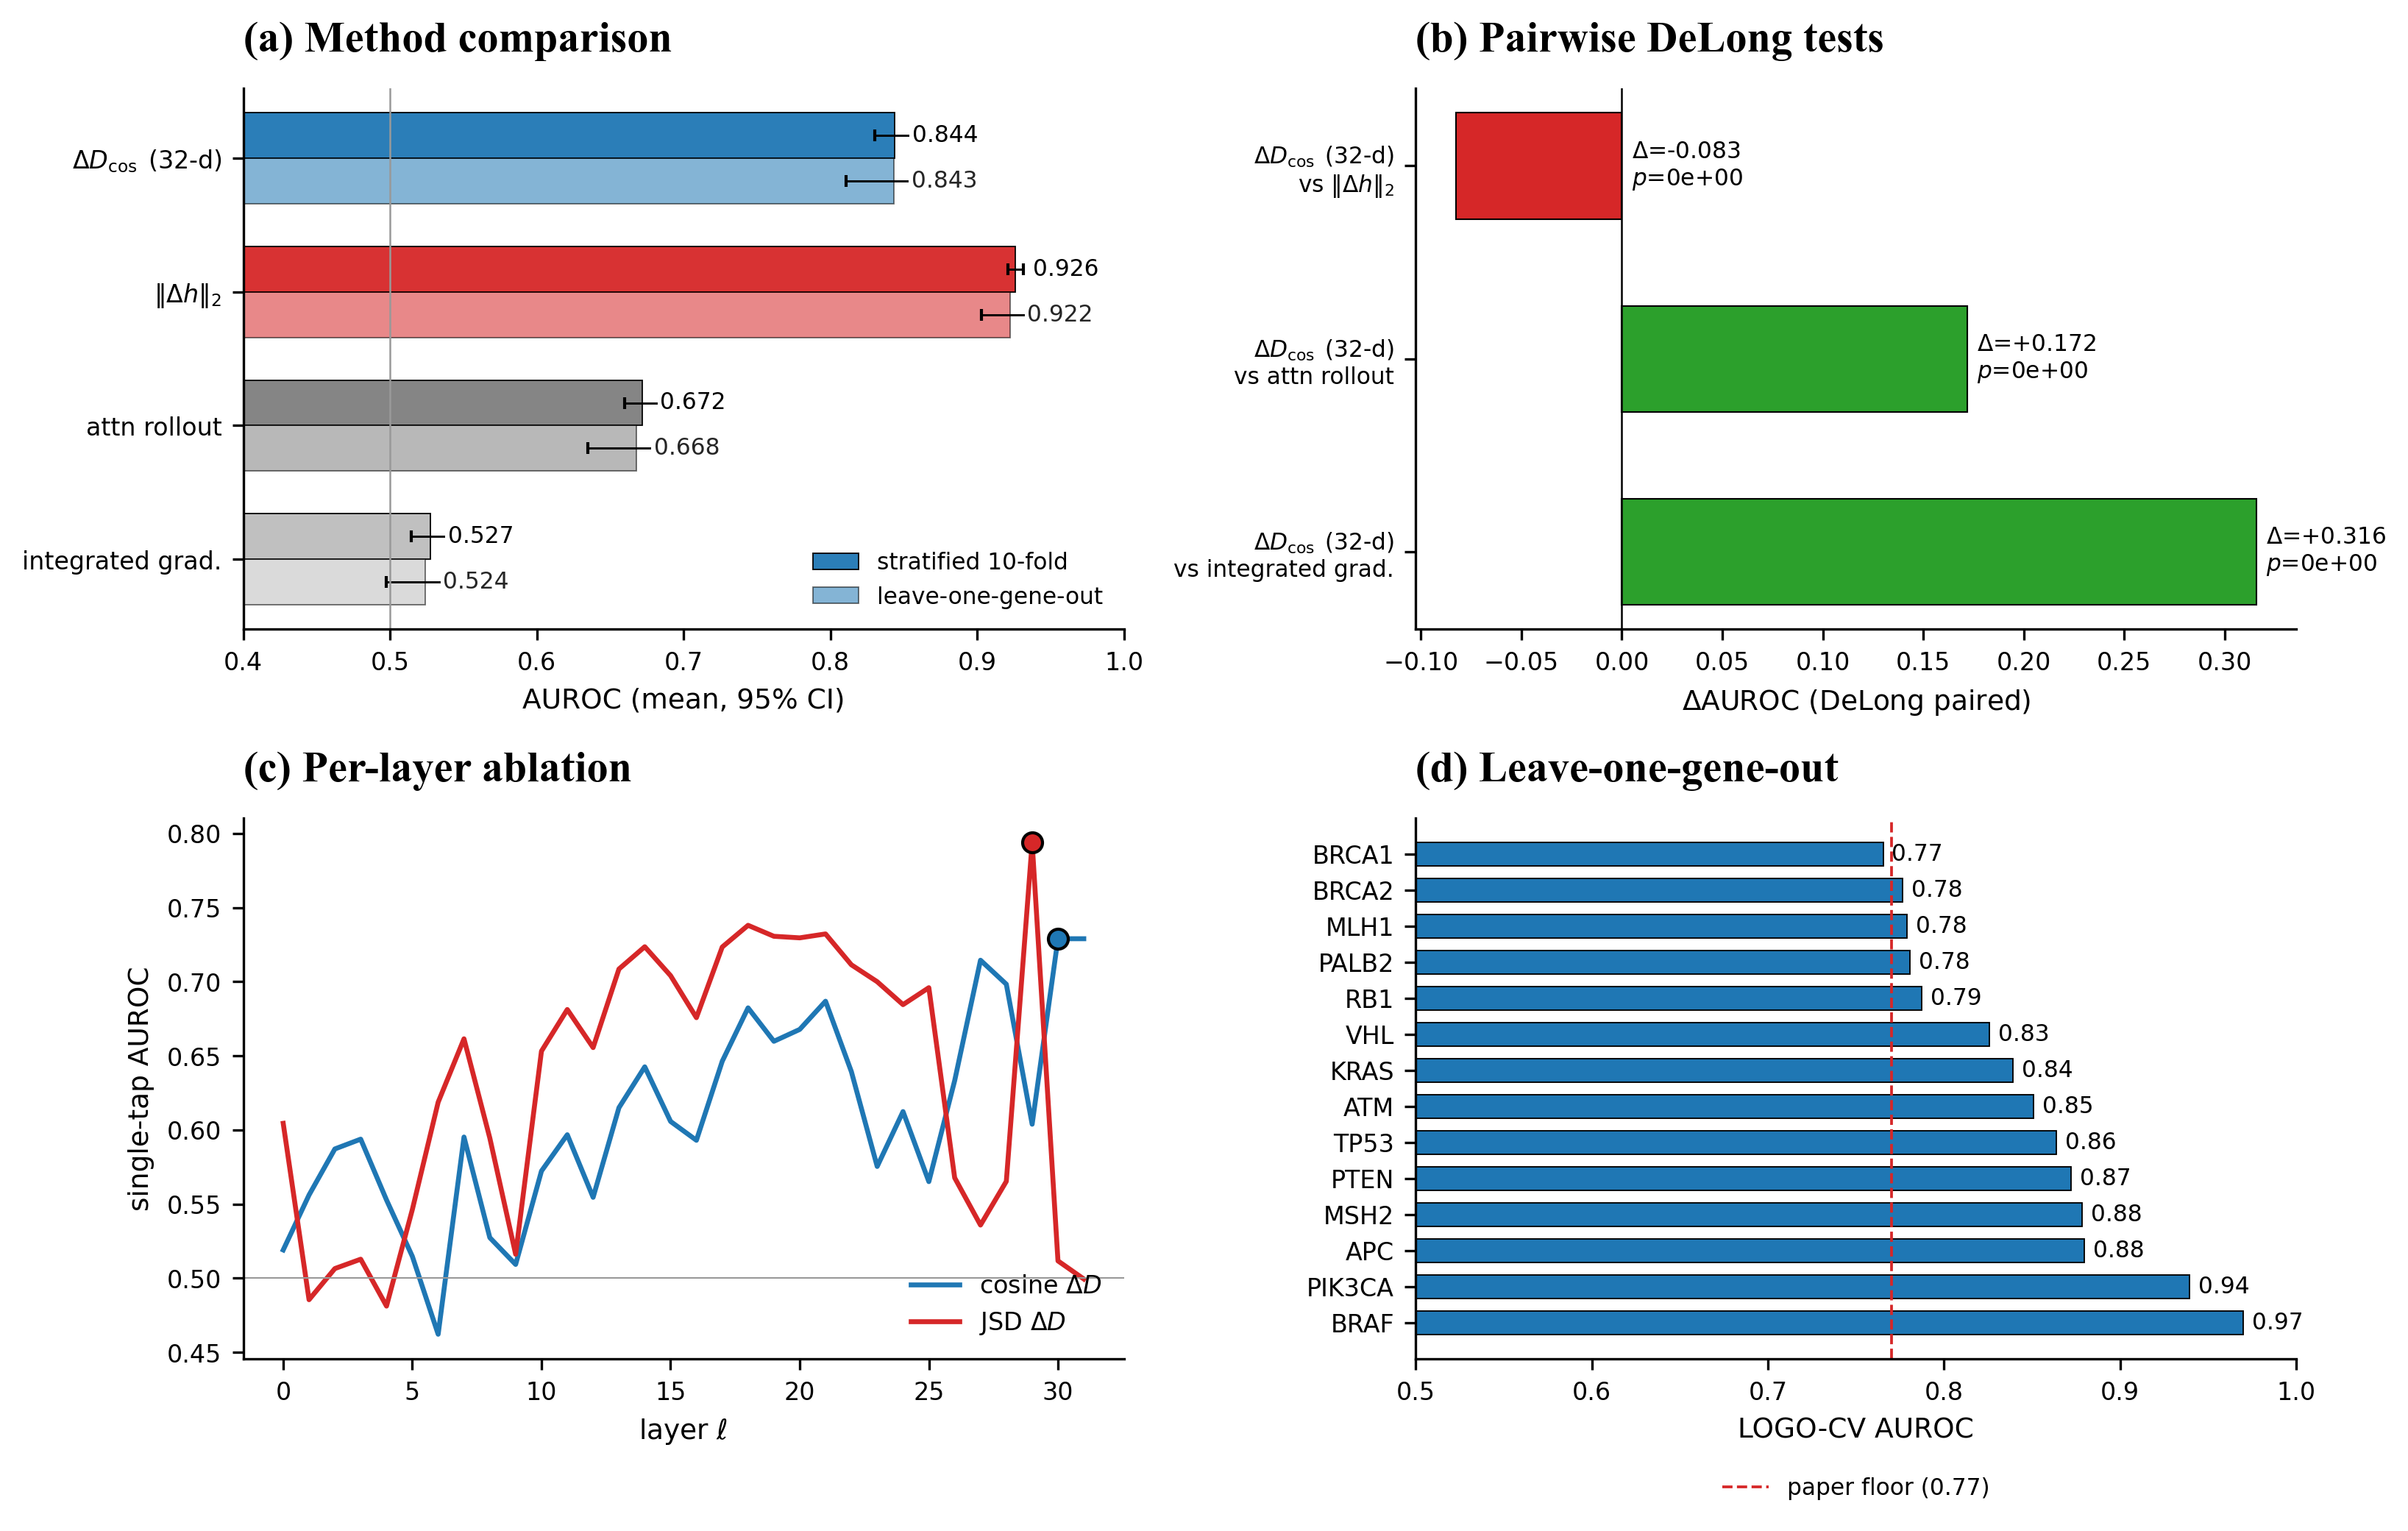
\includegraphics[width=0.95\linewidth]{figures/fig_A3_auroc.png}
  \caption{Variant pathogenicity discrimination on $8{,}008$ ClinVar
    P/LP vs B/LB SNVs across 15 cancer-associated genes (numerical summary
    in Table~\ref{tab:auroc}). \textbf{(a)}~ROC curves for the four scoring
    features. \textbf{(b)}~Paired DeLong tests: $\Delta D$ adds
    significant information beyond Evo~2 $\Delta\textrm{LL}$
    ($p\!=\!3.6\!\times\!10^{-15}$). \textbf{(c)}~Per-layer single-feature
    AUROC across all 32 layers -- best single tap is $\ell\!=\!29$ for JSD
    and $\ell\!=\!30$ for cosine (the latter is the post-norm rotation
      block, not the canonical interpretive tap; see
    App.~\ref{app:architectural-quirk}); the 32-d vector beats either by
    $+0.05$ to $+0.12$.
    \textbf{(d)}~Leave-one-gene-out AUROC across 14 evaluable genes is
  uniformly high ($\ge 0.77$).}
  \label{fig:auroc}
\end{figure}

%%%%%%%%%%%%%%%%%%%%%%%%%%%%%%%%
% APPENDIX D — Splice anatomy beyond the headline contexts
% (merged: positional fine-profile + canonical-vs-non-canonical motifs)
%%%%%%%%%%%%%%%%%%%%%%%%%%%%%%%%
\section{Splice Anatomy Beyond the Headline Contexts}
\label{app:splice-anatomy}

This appendix supports the cautionary message in
\S\ref{sec:motif-controls}: the splice signal is real, but its internal
structure is asymmetric and motif-class-dependent.

\subsection{Positional Fine-Profile Around Donor / Acceptor}
\label{app:splice-fine}

On chr17 the donor profile reaches its mean settling-depth minimum at
position $+20$\,bp ($\bar c\!=\!24.06$) and remains $\ge 1.5$ layers
below intronic baseline ($\bar c\!=\!27.69$) out to $\pm 200$\,bp. On
the same chromosome the acceptor profile reaches its minimum at
$+50$\,bp ($\bar c\!=\!23.33$) and similarly remains depressed beyond
$\pm 200$\,bp. On chr22 both donor and acceptor minima sit at coordinate
$0$ ($\bar c\!=\!23.65$ and $23.64$ respectively). The asymmetry --- donor
minimum exonic-side, acceptor minimum intronic-side --- mirrors the
asymmetric splice-grammar features (branch point, polypyrimidine tract)
that lie predominantly on the intronic side of acceptors. The full
positional profile is shown in Fig.~\ref{fig:splice-fine}; the per-side
minima are summarised in Table~\ref{tab:splice-fine}.

\begin{figure}[!htbp]
  \centering
  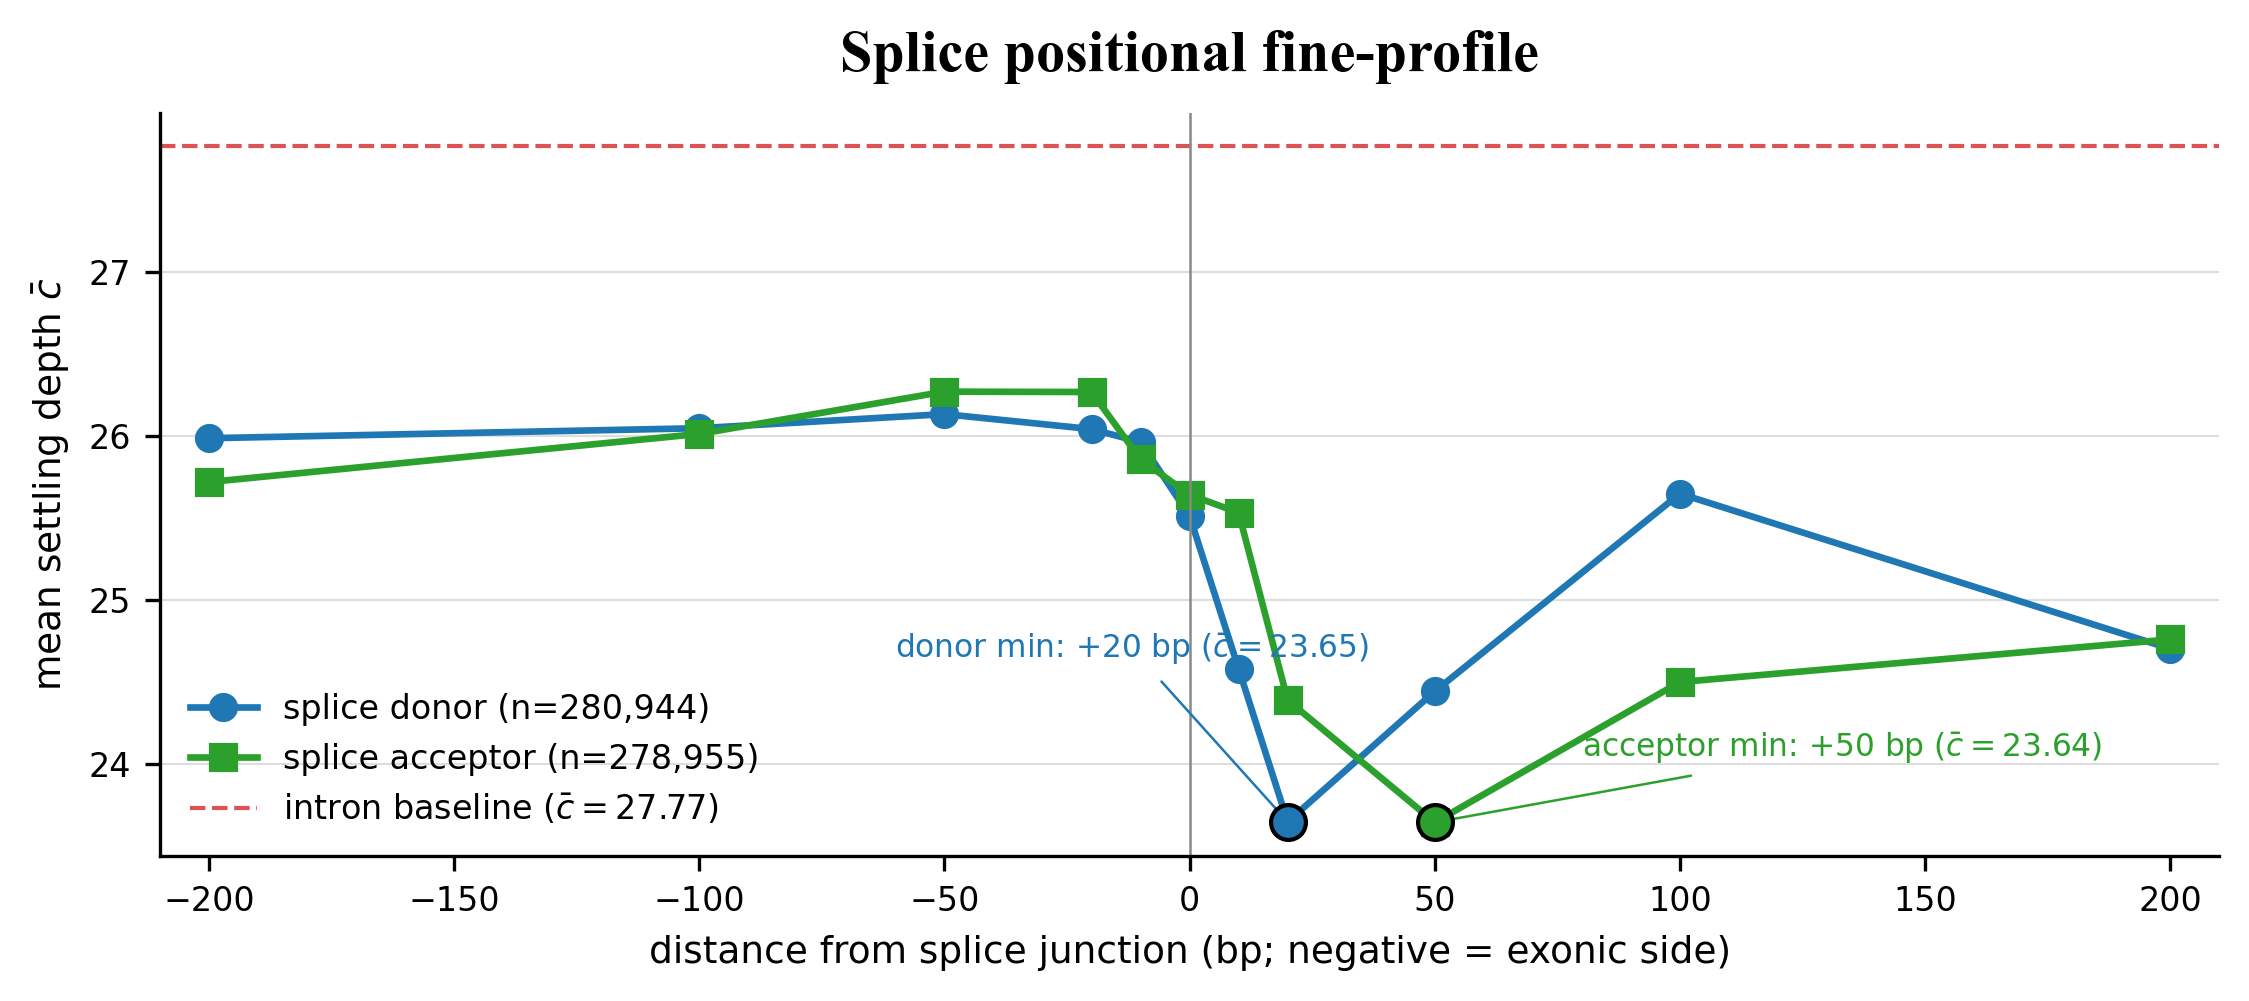
\includegraphics[width=0.95\linewidth]{figures/fig_A4_splice_fine.png}
  \caption{Mean settling depth $\bar c$ as a function of distance to the
    nearest splice donor / acceptor, computed on the pooled chr17 + chr22
    analysis windows. Both profiles dip well below the intronic baseline
    ($\bar c\!=\!27.72$, red dashed) within $\pm 200$\,bp; donors minimise
    on the exonic side, acceptors on the intronic side, mirroring the
    asymmetric splice-grammar context (branch point and polypyrimidine
  tract on the intronic side of acceptors).}
  \label{fig:splice-fine}
\end{figure}

\begin{table}[!htbp]
  \caption{Per-side minima of the splice positional fine-profile.
    Pooled chr17 + chr22 analysis windows; positions measured from the
    splice junction. Donor exonic-side / acceptor intronic-side minima
  recapitulate the asymmetric splice-grammar context.}
  \label{tab:splice-fine}
  \centering
  \small
  \begin{tabular}{@{}lccccc@{}}
    \toprule
    Side & arg-min position & $\bar c$ at min & $\bar c$ at $-100$\,bp
    & $\bar c$ at $+100$\,bp & $n$ \\
    \midrule
    splice donor    & $+20$\,bp & $23.65$ & $26.05$ & $25.65$ & $280{,}944$ \\
    splice acceptor & $+50$\,bp & $23.64$ & $26.01$ & $24.50$ & $278{,}955$ \\
    \bottomrule
  \end{tabular}
\end{table}

\subsection{Canonical vs.\ Non-Canonical Splice Motif Breakdown}
\label{app:splice-canonical}

A finer dissection by motif class -- using the genomic dinucleotides
immediately downstream of the donor and upstream of the acceptor ---
reveals an unexpected ordering (Table~\ref{tab:splice-canonical}):
\emph{non-canonical} splice donors converge \emph{earlier} than the
dominant canonical GT-AG donors, while the minor canonical GC-AG class
is the deepest of the three. The shallower-than-intron pattern
($\bar c\!=\!27.72$) holds for every splice class, but the within-class
ordering is the opposite of a naive ``stronger motif $\Rightarrow$
shallower recognition'' prior. The Cohen's $d$ between canonical GT-AG
and non-canonical donors is small ($\approx 0.05$), consistent with the
constrained branch-point and polypyrimidine context that flanks
non-canonical introns~\cite{wang2008splicecode,burge1998u12}; we
report the magnitudes honestly rather than over-interpret. The finding
replicates qualitatively on the 8-layer HyenaDNA-large at depth-normalised
scale.

\begin{table}[!htbp]
  \caption{Within-splice motif breakdown by donor dinucleotide. The
    shallower-than-intron pattern ($\bar c\!=\!27.72$) holds for every
    splice class, but the within-class ordering is the opposite of a naive
    ``stronger motif $\Rightarrow$ shallower recognition'' prior:
  non-canonical donors converge earliest, GC-AG latest.}
  \label{tab:splice-canonical}
  \centering
  \small
  \begin{tabular}{@{}lccc@{}}
    \toprule
    Donor motif class & $n$ & $\bar c$ & vs.\ canonical GT-AG \\
    \midrule
    non-canonical (AT-AC, other) & $\phantom{00}5{,}977$ & $25.13$ & $d\approx -0.05$ (shallower) \\
    canonical GT-AG (dominant)   & $350{,}552$ & $25.79$ & --- (reference) \\
    canonical GC-AG (minor)      & $\phantom{00}5{,}165$ & $27.01$ & $d\approx +0.10$ (deeper) \\
    \midrule
    intron baseline              & $\sim\!10^7$           & $27.72$ & --- (deeper than every class) \\
    \bottomrule
  \end{tabular}
\end{table}

\subsection{Motif and Flank Perturbation Summary}
\label{app:motif-flank}

Table~\ref{tab:motif-flank} summarises the motif-edit and flank-shuffle
controls of \S\ref{sec:motif-controls}. On $1{,}000$ canonical GT-AG
donors (chr22, $\pm 10$\,bp pad-averaged $c$) the central GT motif
contributes a small but reliable detection signal ($\bar c$ deepens by
$0.46$ layers when GT is replaced with AA), whereas dinucleotide-shuffling
the $\pm 100$\,bp flank lifts $\bar c$ to a shallower value by $3.18$ layers, isolating the
GT for easier stabilisation. Real flanking grammar therefore demands
deeper integration than the central motif on its own.

\begin{table}[!htbp]
  \caption{Motif-edit and flank-shuffle controls on 1{,}000 canonical
    GT-AG donors. Real $\bar c\!=\!26.77$. Replacing the central GT with AA
    (while keeping the flank) deepens $\bar c$; shuffling the flank
  (while keeping GT) \emph{lifts} $\bar c$ to a shallower value by 3.18 layers.}
  \label{tab:motif-flank}
  \centering
  \small
  \begin{tabular}{@{}lcccc@{}}
    \toprule
    Condition & $\bar c$ & $\Delta \bar c$ vs.\ real & Cohen's $d$ & paired Wilcoxon $p$ \\
    \midrule
    real GT-AG donor (reference)             & $26.77$ & $0$ (ref.)   & ---     & --- \\
    GT $\to$ AA, flank preserved             & $27.24$ & $+0.46$      & $-0.086$ & $2.3\!\times\!10^{-32}$ \\
    GT preserved, $\pm 100$\,bp flank shuffled & $23.59$ & $\mathbf{-3.18}$ & $\mathbf{+0.515}$ & $4.1\!\times\!10^{-59}$ \\
    \bottomrule
  \end{tabular}
\end{table}

%%%%%%%%%%%%%%%%%%%%%%%%%%%%%%%%
% APPENDIX E — Reproducibility (now last)
%%%%%%%%%%%%%%%%%%%%%%%%%%%%%%%%
\section{Reproducibility}
\label{app:repro}

All experiments use random seed $42$ for cross-validation splits and
bootstrap resamples. The Evo~2 model lock is
\texttt{arcinstitute/evo2\_7b} at HF revision SHA
\texttt{bda0089f92582d5baabf0f22d9fc85f3588f6b58} (weights MD5
\texttt{359ef88ccac2a62644035578de8a7db4}). Data versions:
GRCh38 primary assembly (UCSC, MD5 locked); GENCODE v44 GTF
(per-chromosome filtered, persisted as \texttt{gffutils} SQLite);
PhyloP 100-way (UCSC); ENCODE SCREEN v3 cCRE catalog with ELS subset;
RepeatMasker hg38; GTEx v8 cis-eQTL pairs (\texttt{Whole\_Blood,
Brain\_Cortex, Liver, Lung} unioned); GWAS Catalog v1.0; ClinVar
2026-04-18. Software stack: \texttt{torch 2.4.1+cu124, evo2 0.3.0,
  vortex 1.0.8, transformer-engine 2.14.0, transformers 4.49.0, scipy
1.13, scikit-learn 1.4}. Hardware: a single NVIDIA H200 (141\,GB).
Total compute: $\sim 20$ GPU-hours end-to-end. Code, dataset version
locks, and figure-generation scripts will be released at an anonymous
URL upon acceptance (an anonymized repository is provided as
supplementary material for review).

\end{document}
